%% LyX 2.3.5.2 created this file.  For more info, see http://www.lyx.org/.
%% Do not edit unless you really know what you are doing.
\documentclass[english]{article}
\usepackage[T1]{fontenc}
\usepackage[latin9]{inputenc}
\usepackage{geometry}
\geometry{verbose,tmargin=2.5cm,bmargin=2.5cm,lmargin=2.5cm,rmargin=6cm}
\usepackage{babel}
\usepackage{float}
\usepackage{graphicx}
\PassOptionsToPackage{normalem}{ulem}
\usepackage{ulem}
\usepackage[unicode=true]
 {hyperref}

\makeatletter

%%%%%%%%%%%%%%%%%%%%%%%%%%%%%% LyX specific LaTeX commands.
%% Because html converters don't know tabularnewline
\providecommand{\tabularnewline}{\\}

\makeatother

\begin{document}
\textbf{Roll No : }\textbf{\uline{16CKT07 }}

\textbf{Name:}\textbf{\uline{ Ashwin Kumar Karnad}}

\textbf{Total Marks:\_\_\_\_\_\_\_\_}

\textbf{Signature of the Evaluator:}\\


\section*{EXPERIMENT NO: 1 Rolling a Belan on an inclined surface}

\section{Aim of the experiment}
\begin{enumerate}
\item To find the moment of inertia of belan
\item To find the relation ship between rolling time and the inclination
angle
\item To find the coefficient of friction of the surface.
\item To determine if rolling time is dependant of surface friction.
\end{enumerate}

\section{System description}

Consider the inclined plane in figure \ref{fig:Rolling-Cylinder-on}
.

\begin{figure}[H]
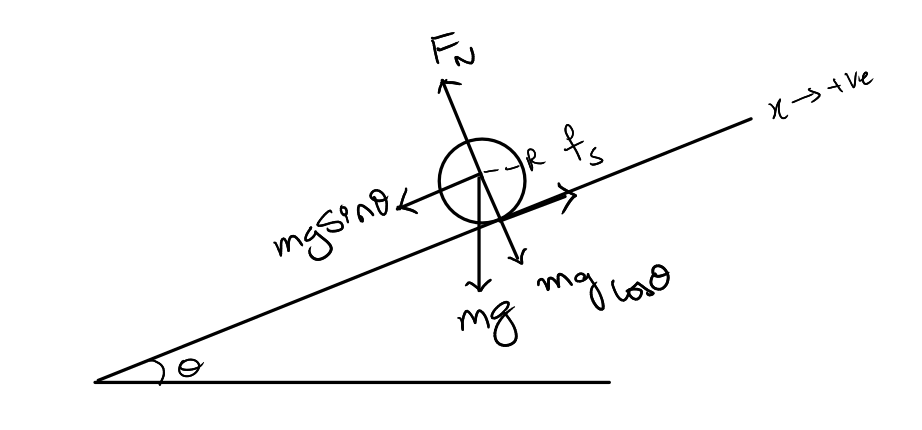
\includegraphics[width=0.4\paperwidth,bb = 0 0 200 100, draft, type=eps]{Fig1.png}

\caption{Rolling Cylinder on an Inclined Plane\label{fig:Rolling-Cylinder-on}}

\end{figure}

let's establish all the forces acting on this rolling body . The force
mg is acting in the downward direction and it has two components one
is parallel to the plank and there's one component which is perpendicular
to the plank and this in turn causes normal reaction and we call it
$F_{n}$ . 

We also have a force of friction which is acting opposite to the direction
of roll. we are considering a situation where the body is not slipping
down the ramp it is smoothly rolling down the lamp so force of friction
which is static in nature is more than $mg\sin\theta$ and it is not
necessary that $f_{s}$ here is $f_{s}max$, so the moment $mg\sin\theta$
exceeds $f_{s}max$ the body will start slipping (i.e for smooth rolling
$f_{s}>mg\sin\theta$)

Lets write the equations of motion of this rolling body, first we'll
write the forces acting on the body considering its linear motion
we can say

\[
f_{s}-mg\sin\theta=ma_{x}
\]

We now notice that only $F_{s}$can produce torque to the body as
all other forces are going right through the axis of rotation of the
cylinder and therefore its distance from the axis of rotation of the
cylinder is zero .

\[
\tau=I\alpha
\]

\[
f_{s}R=I\alpha
\]

\[
a_{x}=R\alpha
\]

\[
f_{s}=Ia_{x}/R^{2}
\]

\[
Ia_{x}/R^{2}-mg\sin\theta=ma_{x}
\]

\[
a_{x}=\frac{g\sin\theta}{1+I/mR^{2}}
\]

The time taken for the cylinder to cover a distance S (along the inclination)
can be calculated from 

\[
t=\sqrt{(\frac{2S}{a_{x}})}
\]

\begin{equation}
t=\sqrt{\frac{2S(1+I/mR^{2})}{g\sin\theta}}\label{eq:time}
\end{equation}

In the limiting case where frictional force can no longer support
rolling of the cylinder, thus the cylinder begins to slip. Analysing
this case, $f_{s}=\mu N=\mu mg\cos\theta$ thus 
\[
\mu mg\cos\theta_{max}=Ia_{x}/R^{2}
\]
 
\[
\mu mg\cos\theta_{max}=\frac{Ig\sin\theta_{max}}{R^{2}+I/m}
\]

\begin{equation}
\mu=\frac{I\tan\theta_{max}}{mR^{2}+I}\label{eq:mu}
\end{equation}


\section{Experimental Method}
\begin{enumerate}
\item Measure the dimensions such as lengths and radii of the Belan and
record them with percentage errors using the accuracy involved with
measuring tools
\item Measure the bench parameters in a similar way.
\item Calculate lift parameters ( vertical lift required for each degree).
\item Lift one end the bench using a Car Jack along with some wooden planks
(ensuring the balance of the bench isn't disturbed).
\item Plot t versus sin$\theta$ other quantities like t2, 1/t, 1/t2 etc.
and try to get a linear plot. 
\item find the moment of inertia of belan.
\item To determine if rolling time is dependant of surface friction.
\item Try find coefficient of friction.
\item Try to replace the surface and determine if rolling time is dependant
of surface.
\end{enumerate}

\section{Observations \& Measurements}

\subsection{Measurement of linear distances}

\subsubsection{Measurement of radii of belan}

In order to measure the radii of the belan, a thread was used cover
the circumference and a marking is done with a pen on both of the
strings at the same level as shown in Fig \ref{fig:Circumference thread}
and then the thread is placed on a ruler and the distance between
the two markings on the string is measured, as shown in Fig \ref{fig:CircumMeasure}
. The least count of scale is 0.05 cm for the smaller radius and 0.1cm
for bigger radius.

\begin{figure}[H]
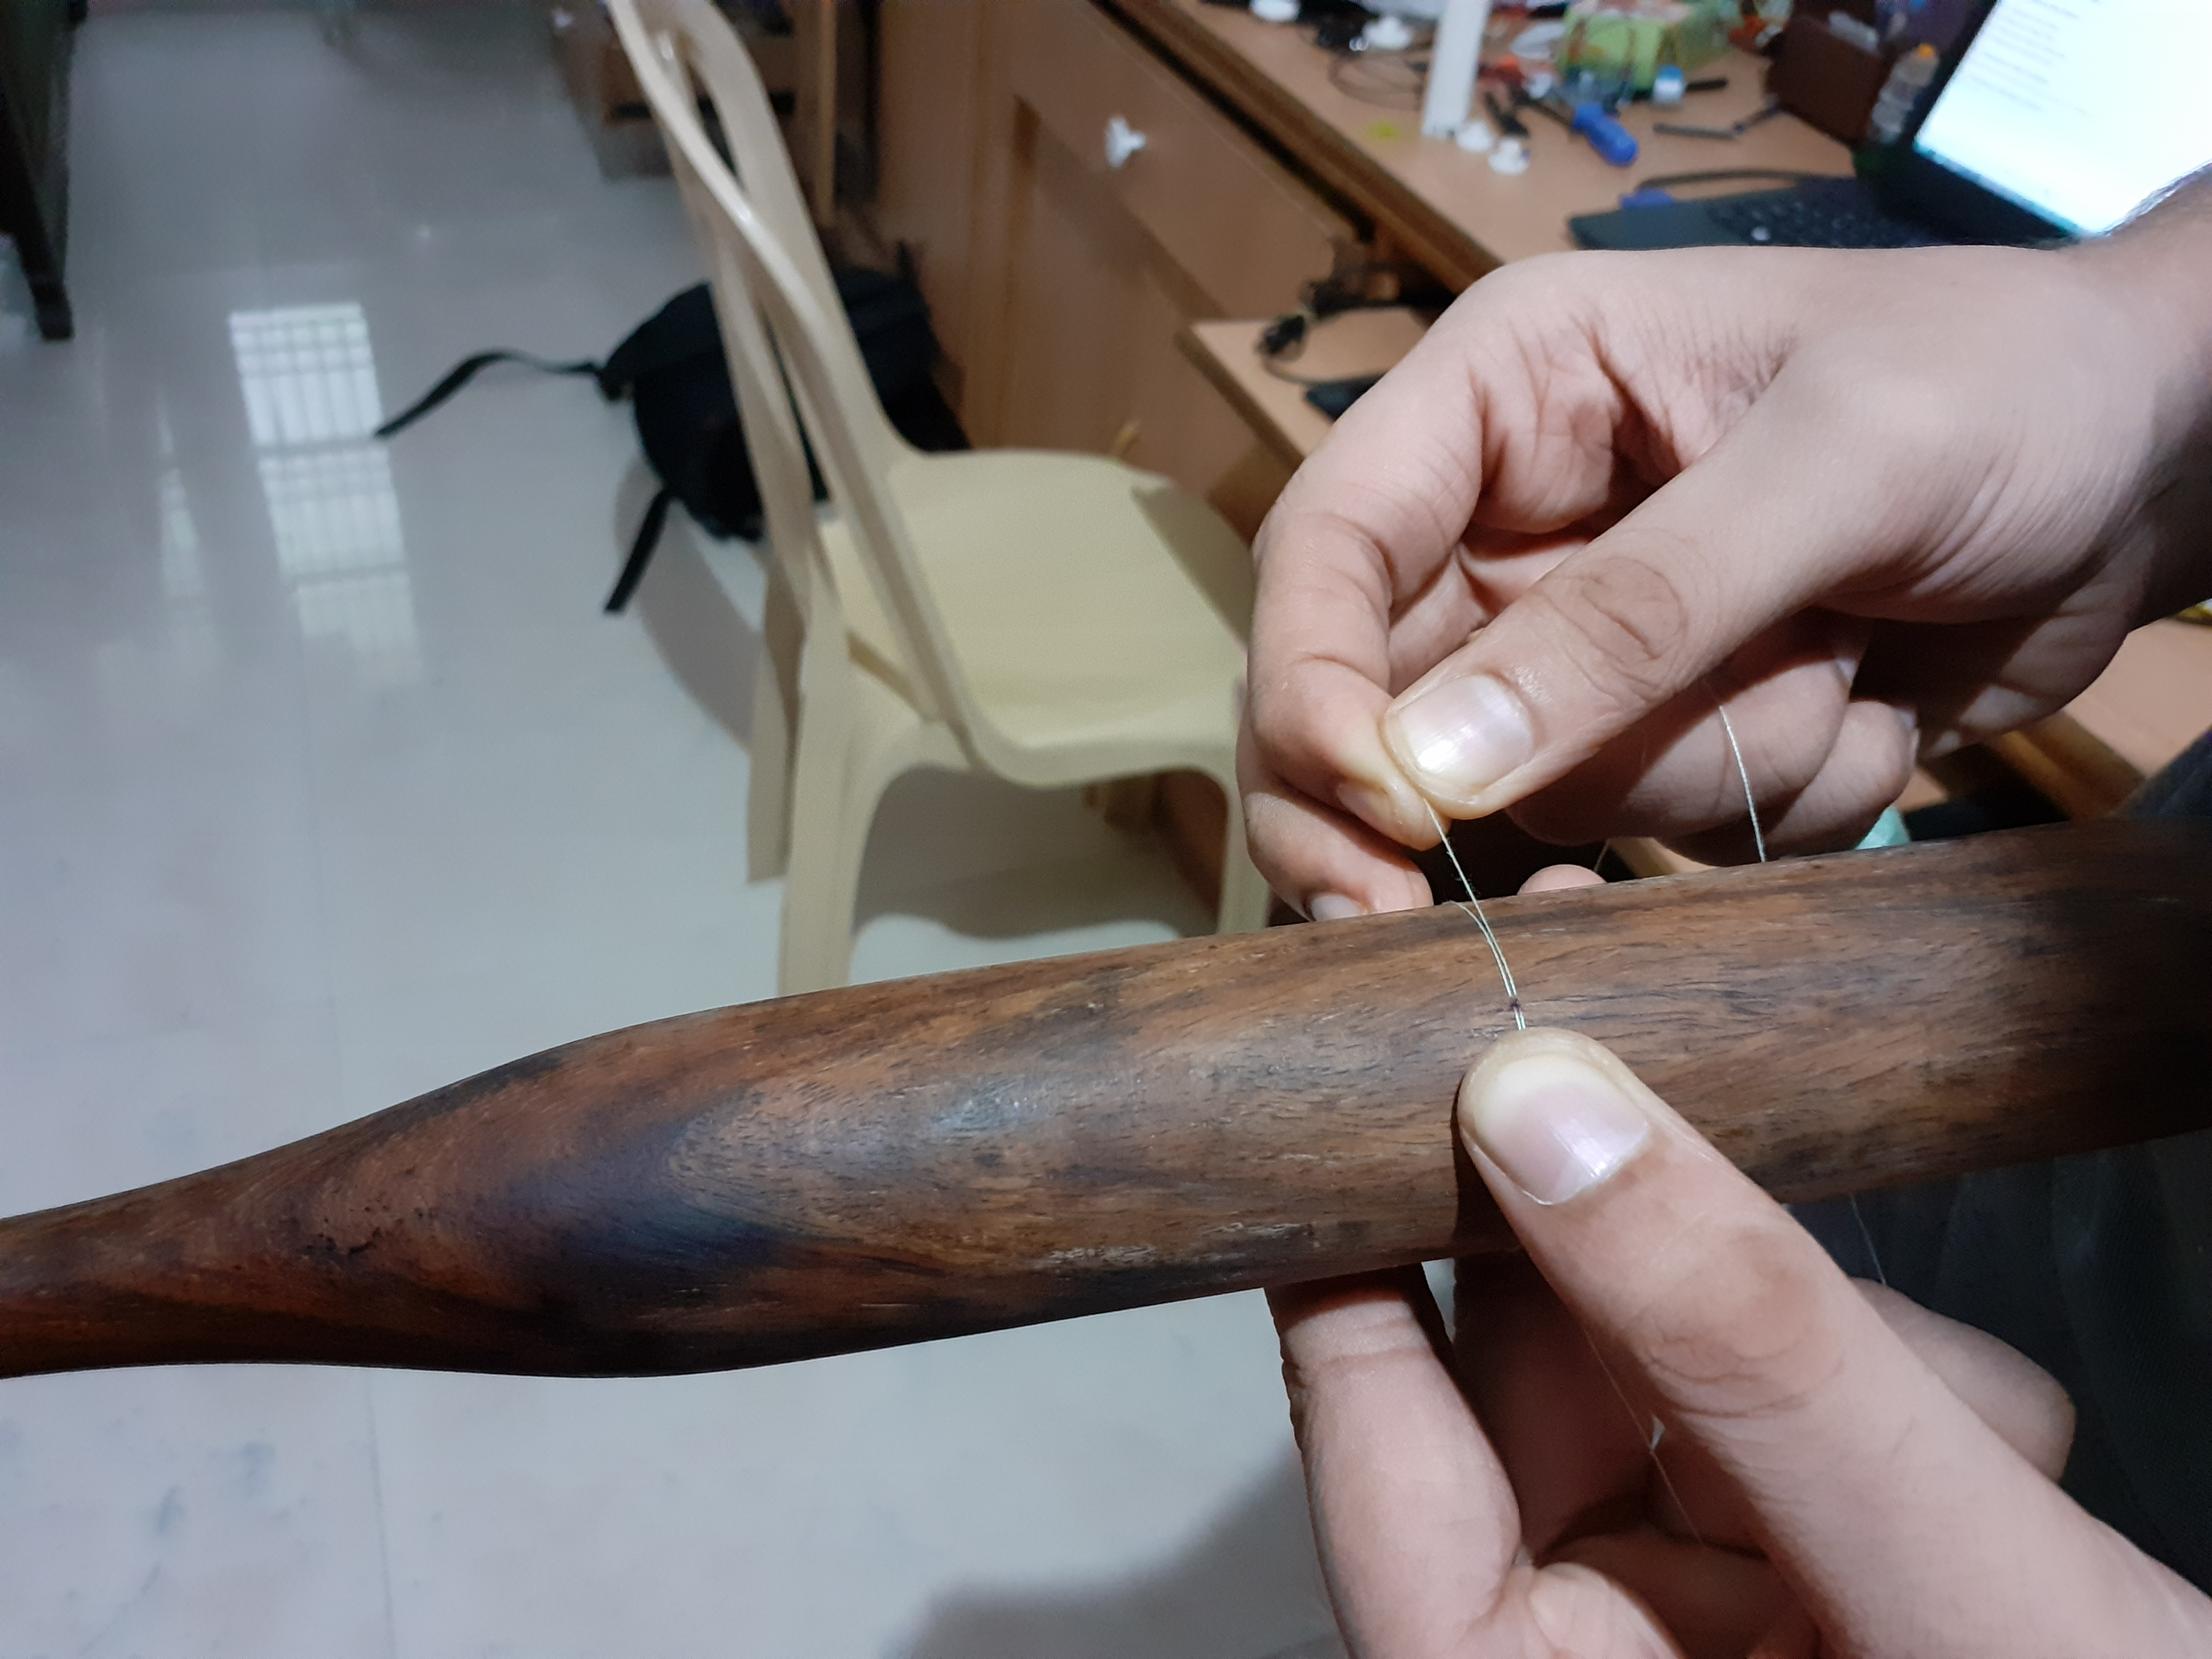
\includegraphics[width=0.4\paperwidth]{Videos/circumferenceig}

\caption{Measuring circumference of larger radius\label{fig:Circumference thread}}
\end{figure}

\begin{figure}[H]
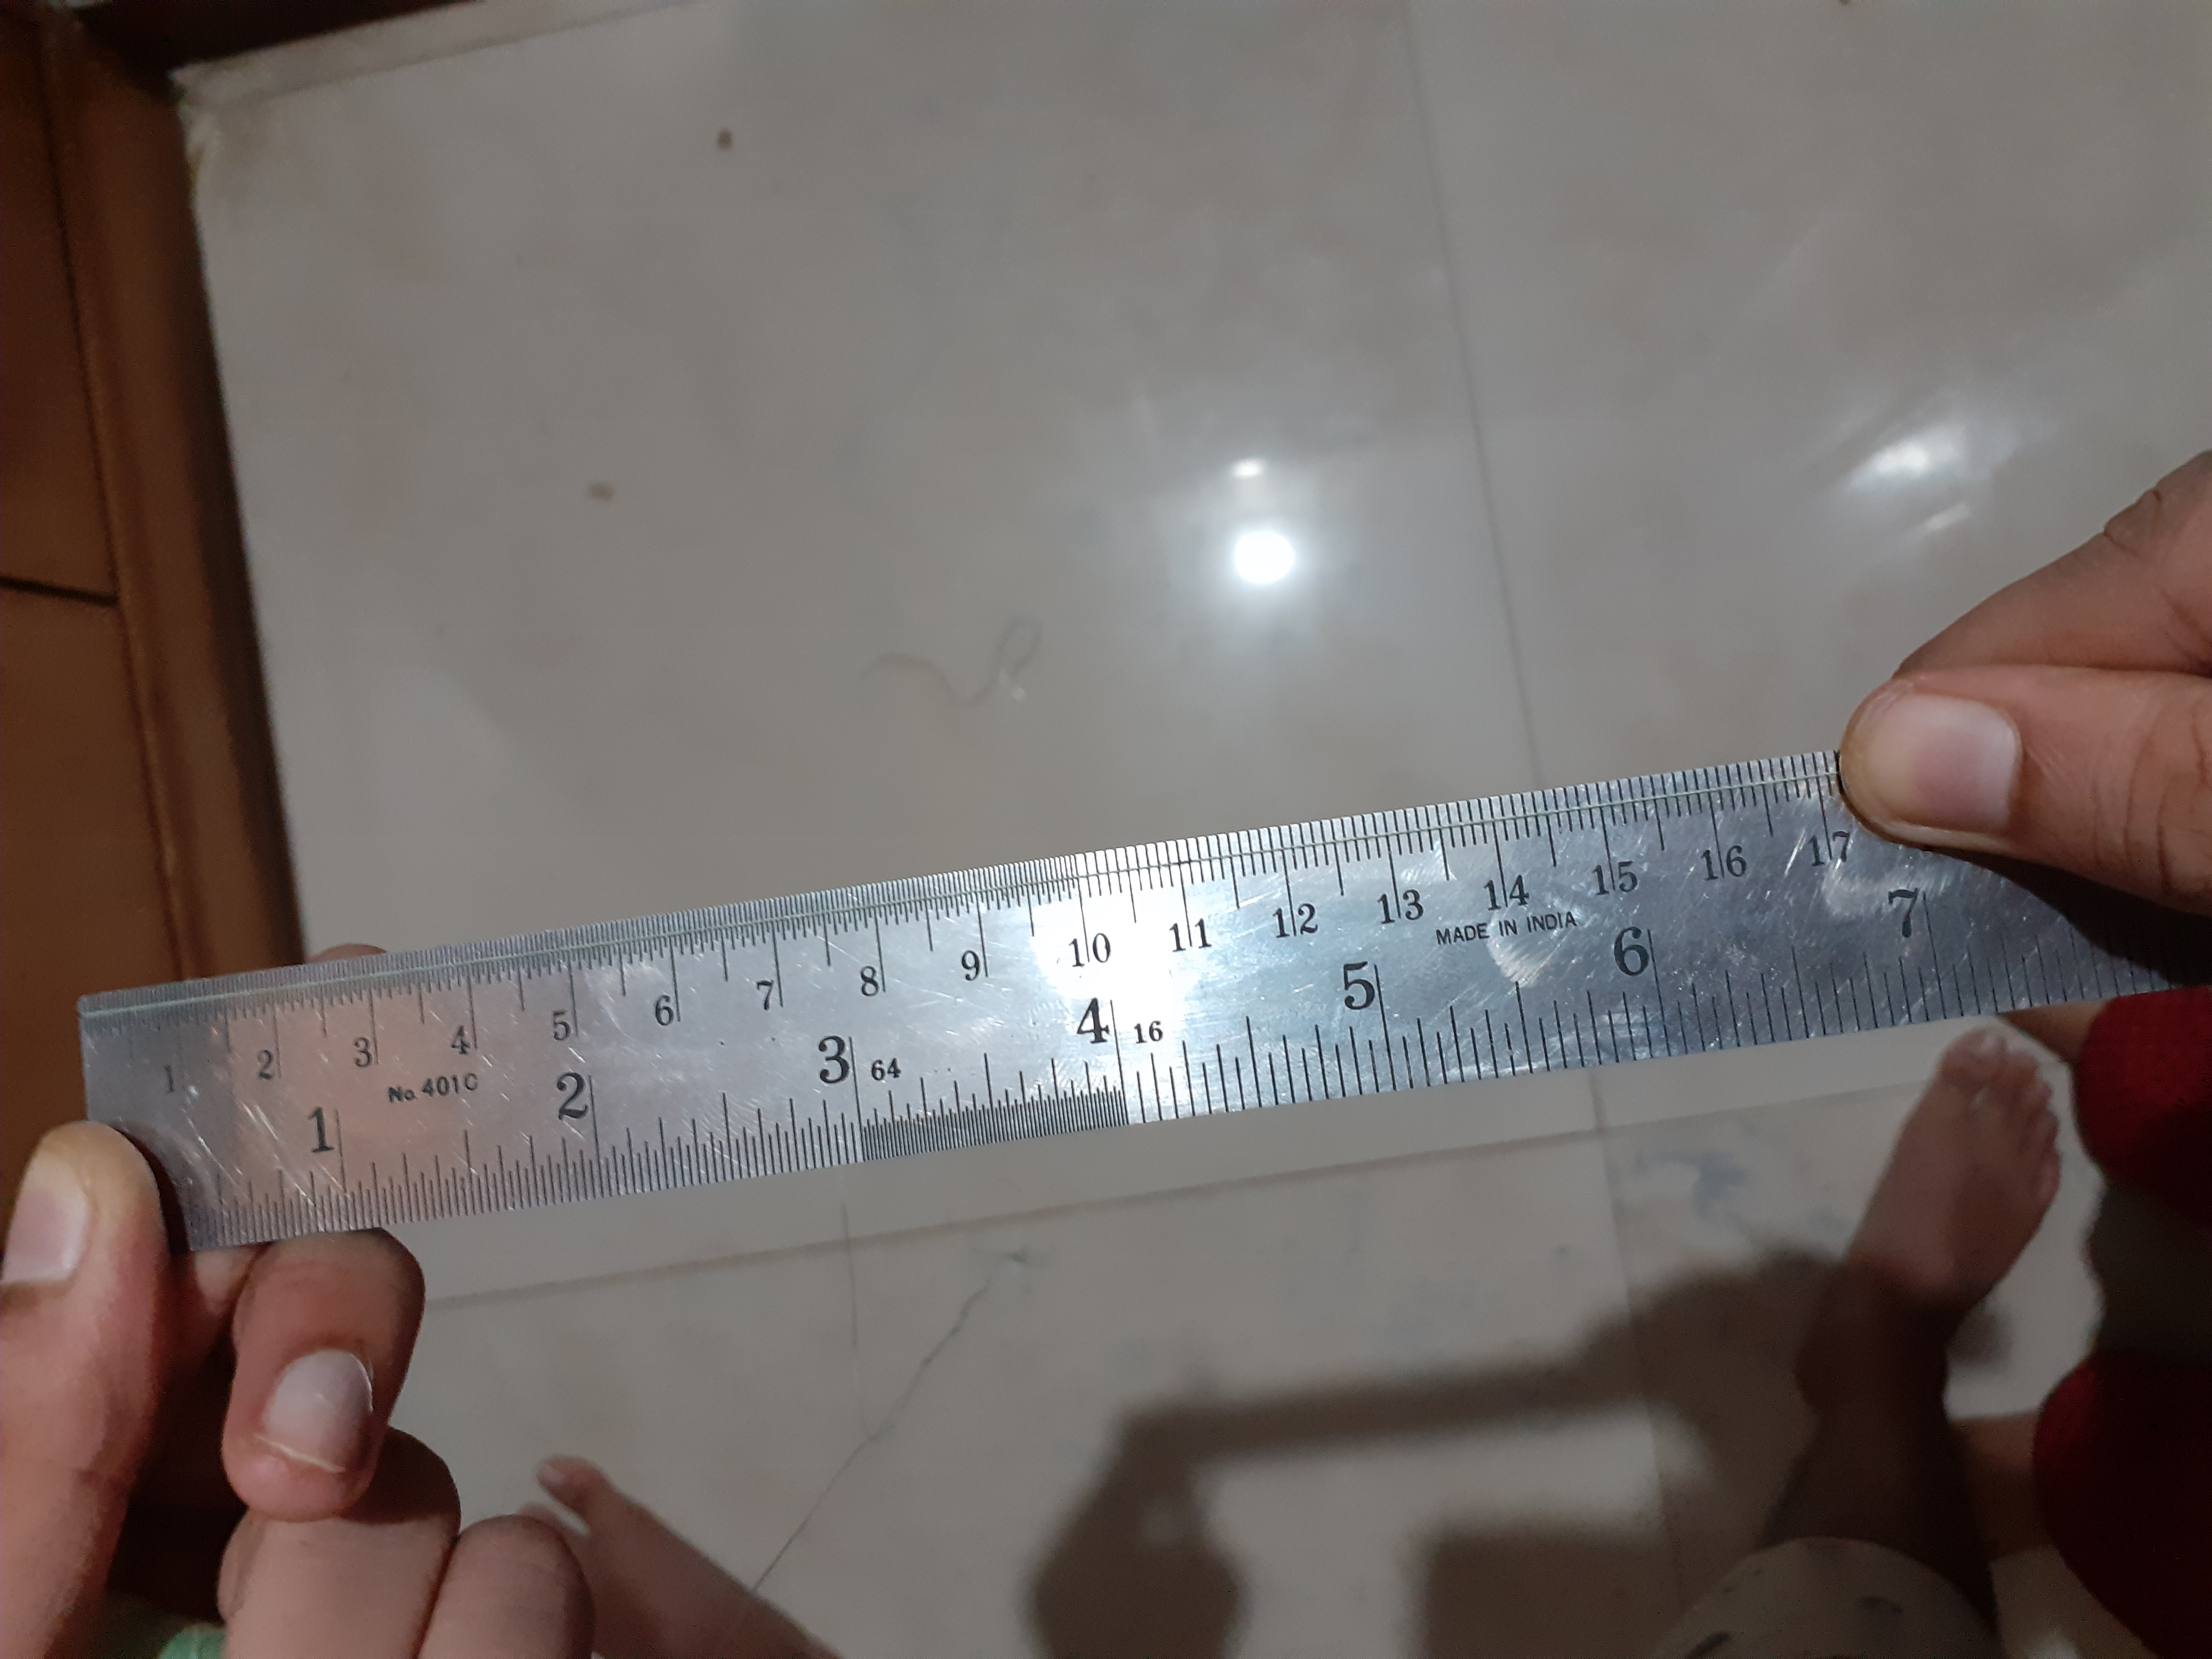
\includegraphics[width=0.4\paperwidth]{Videos/circumMeasureBig}

\caption{Measuring circumference of larger radius\label{fig:CircumMeasure}}
\end{figure}

\begin{figure}[H]
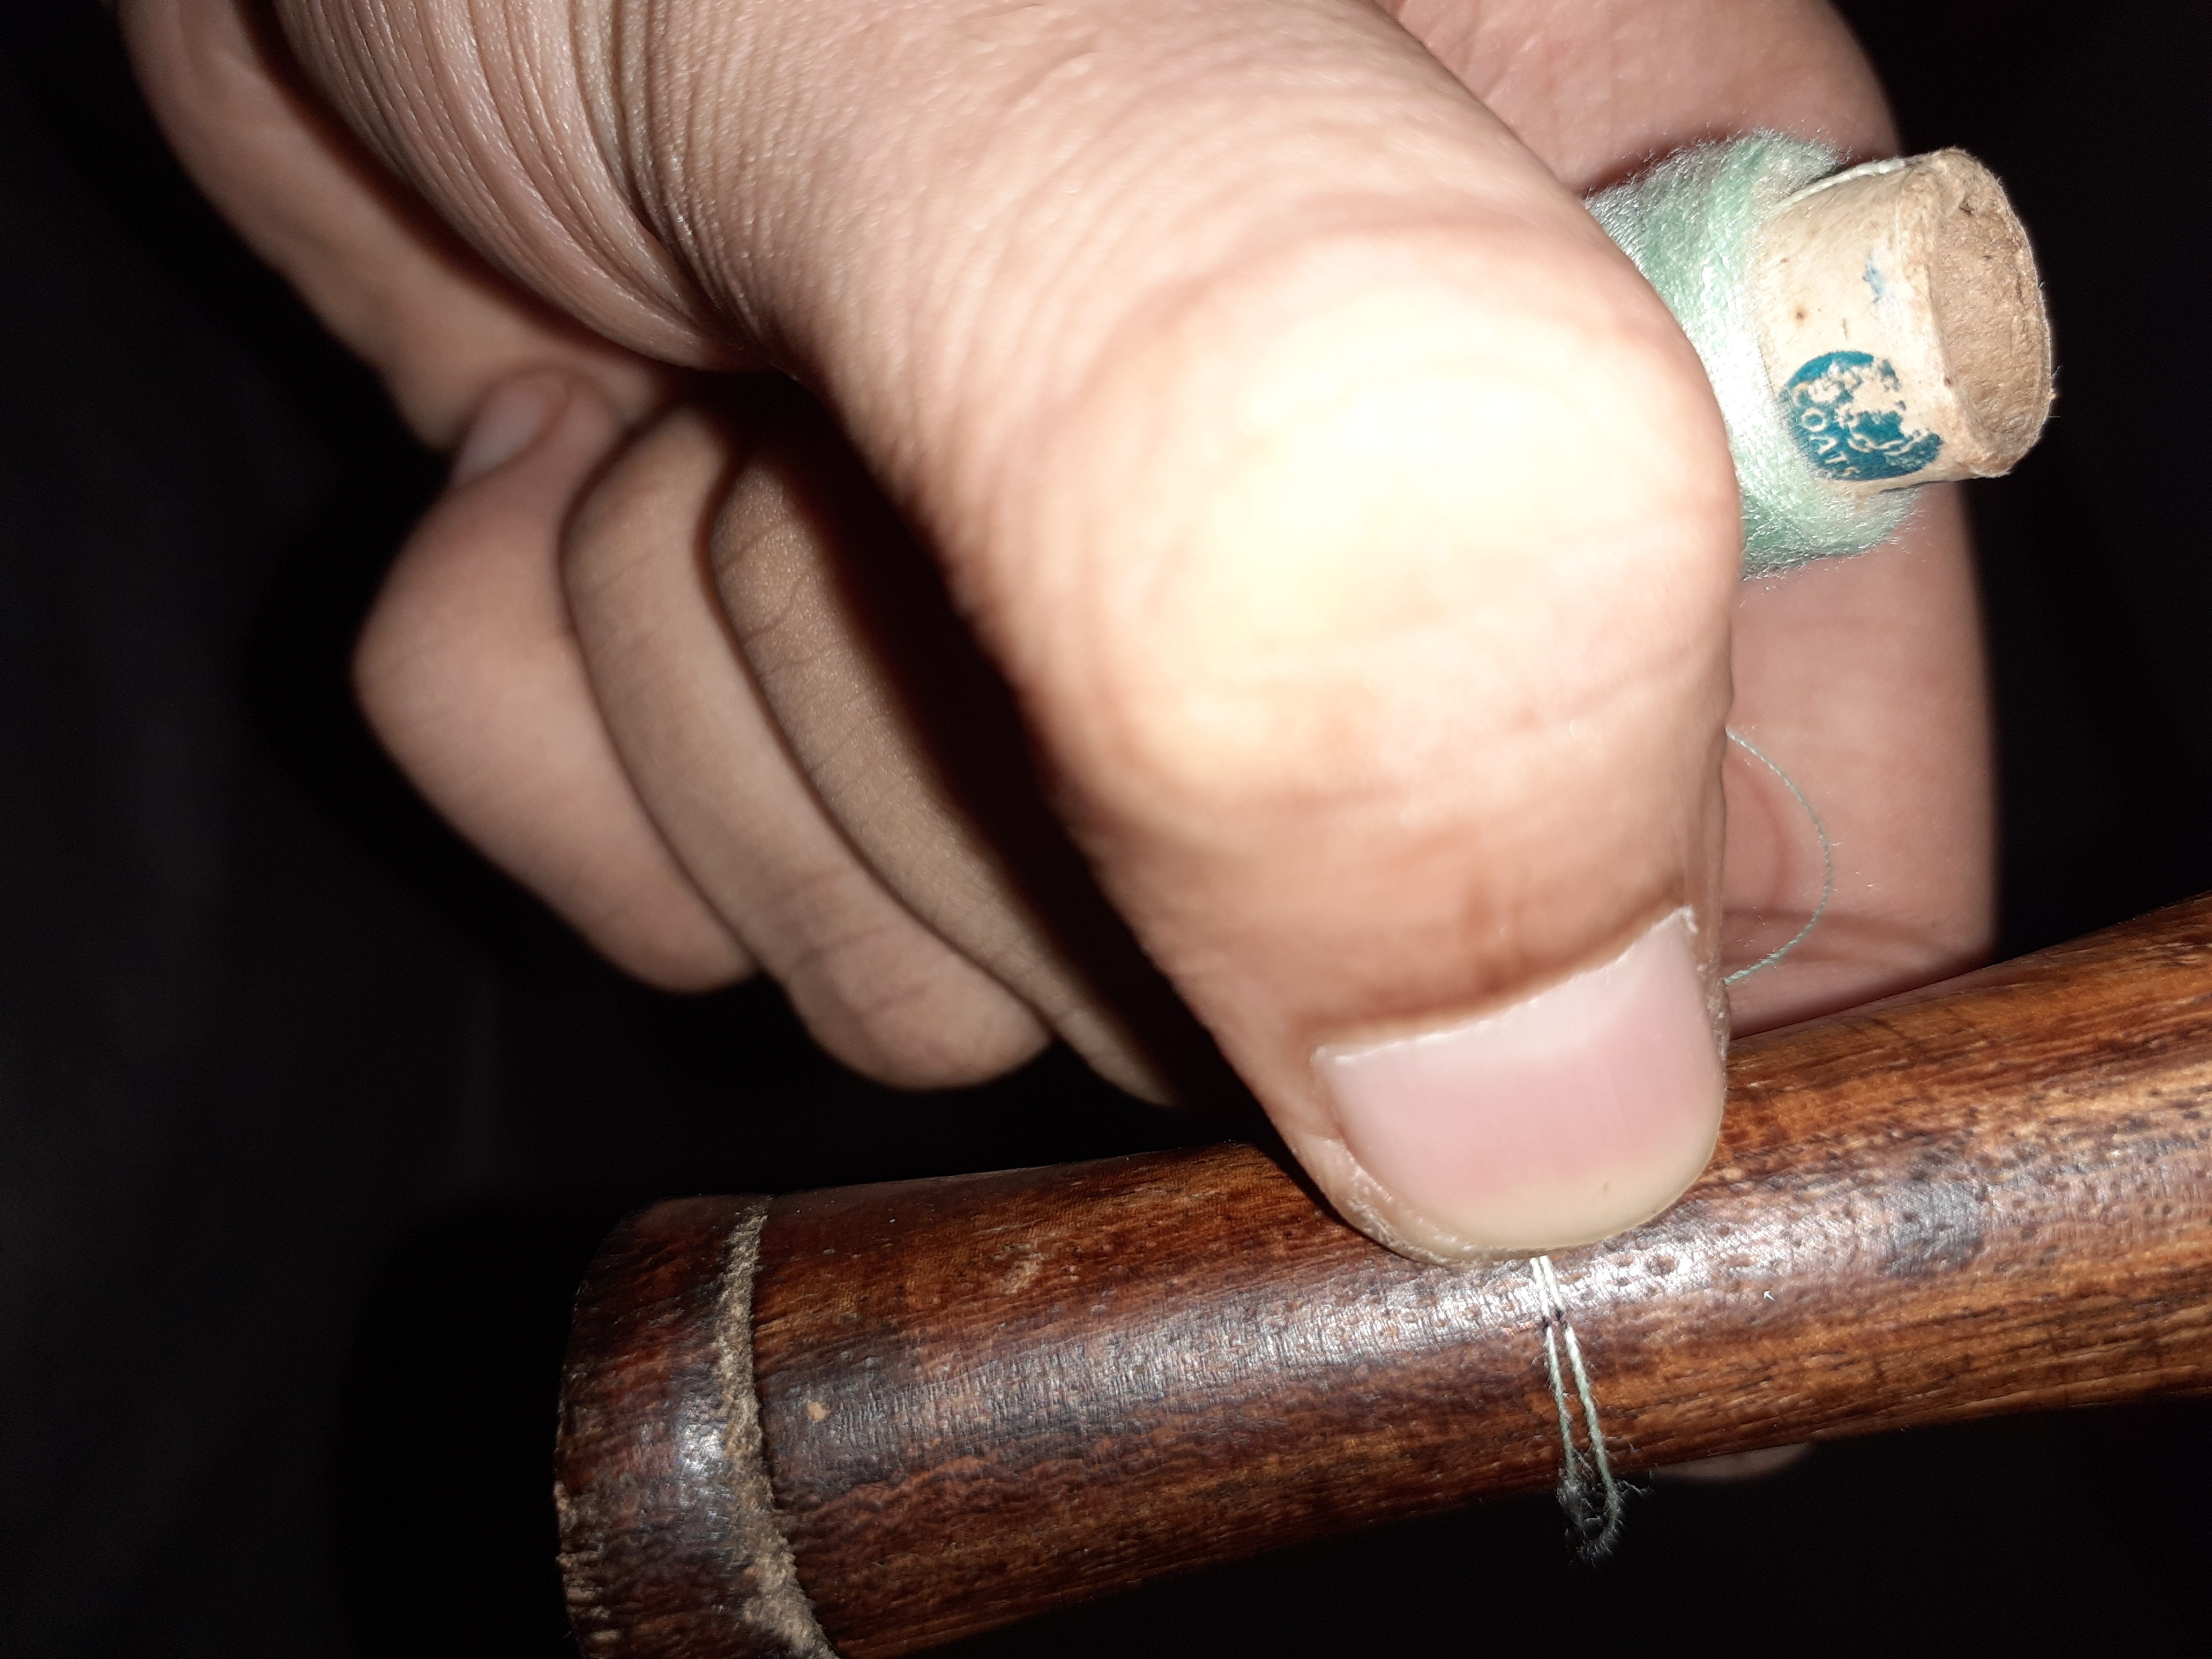
\includegraphics[width=0.4\paperwidth]{Videos/circum_small}

\caption{Measuring circumference of smaller radius\label{fig:Circumference thread-1}}
\end{figure}

\begin{figure}[H]
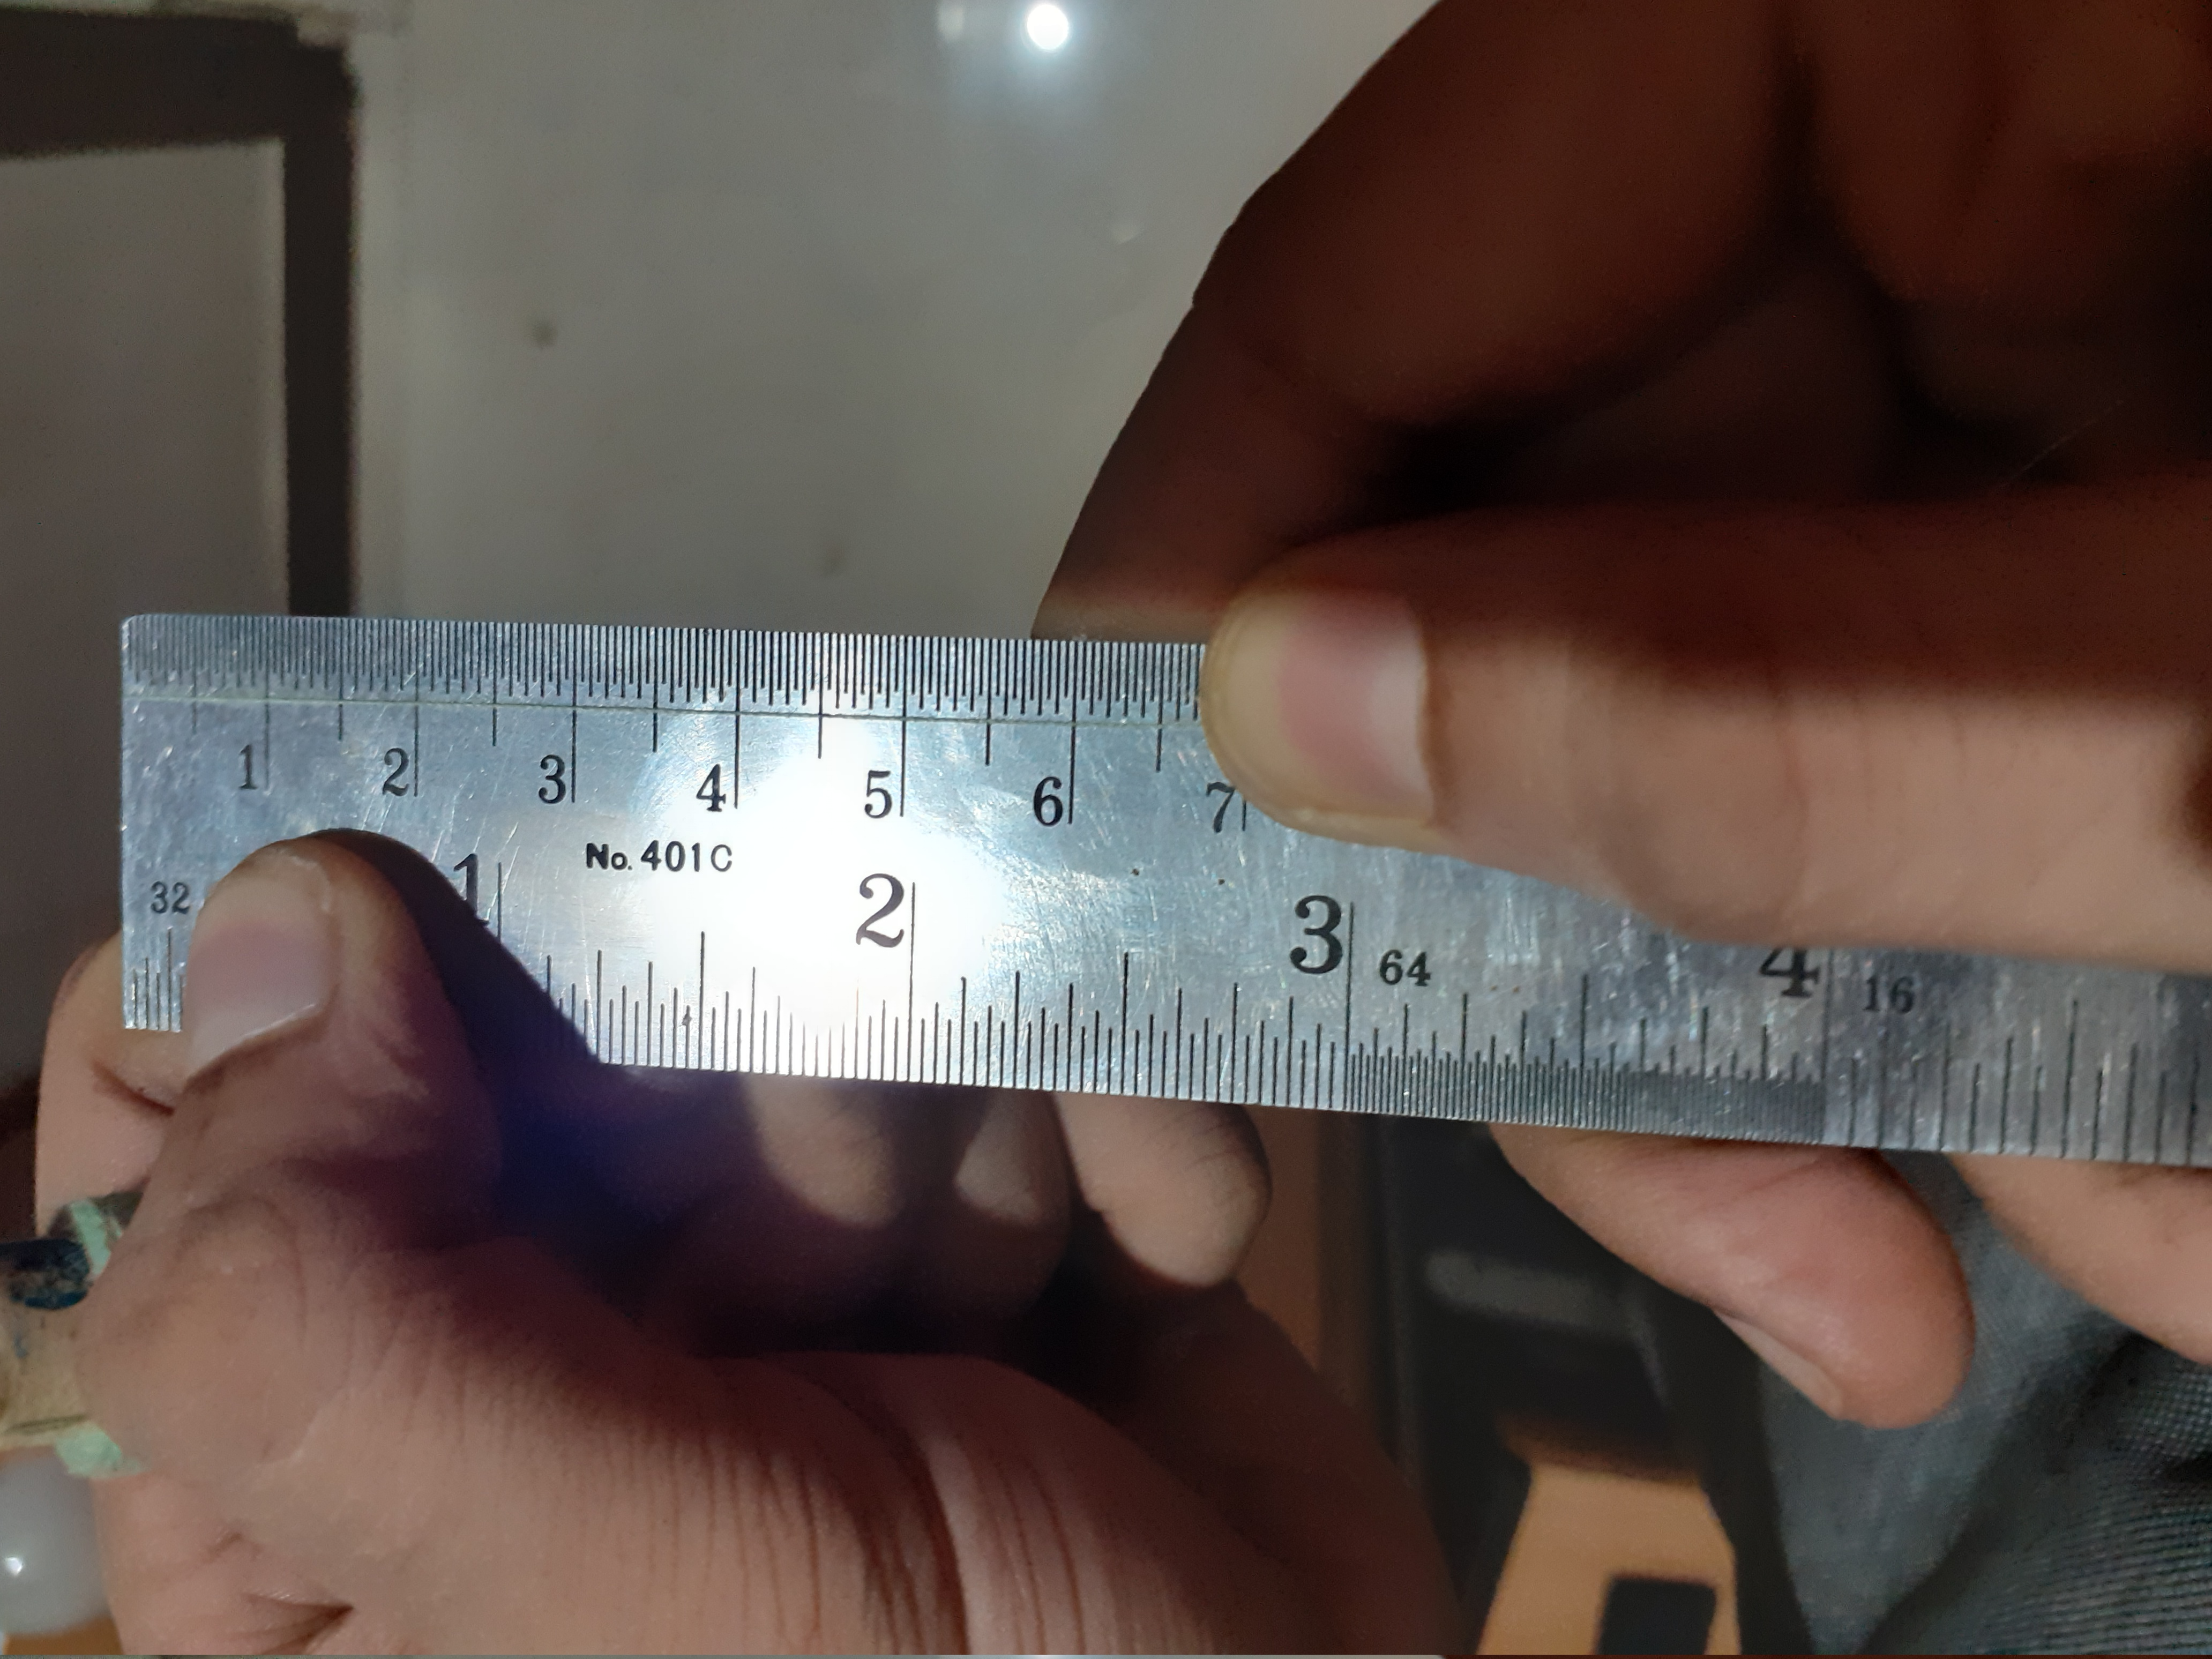
\includegraphics[width=0.4\paperwidth]{Videos/circumMeasureSmall}

\caption{Measuring circumference of smaller radius\label{fig:CircumMeasure-1}}
\end{figure}

\begin{table}[H]
\begin{tabular}{|c|c|c|}
\hline 
 & Circumference of the smaller radius (in cm) & Circumference of the bigger radius (in cm)\tabularnewline
\hline 
\hline 
Trial 1 & 4.5 & 11\tabularnewline
\hline 
Trial 2 & 4.6 & 11.2\tabularnewline
\hline 
Trial 3 & 4.6 & 11.2\tabularnewline
\hline 
Mean value & 4.56 & 11.13\tabularnewline
\hline 
\end{tabular}

\caption{Measured circumference data}

\end{table}

Thus the nominal values of radii are 0.73 cm and 1.77 cm (round to
two decimal places) respectively.

we know that $c=2\pi r$so, $\Delta r=r\Delta c/c$ so the error in
measurement of radius is 0.008 cm and 0.016 cm respectively.

Therefore $R_{1}=0.73\pm0.01$cm and $R_{2}=1.77\pm0.02$cm (two significant
figures).

\subsubsection{Measurement of length of belan}

In order to measure the length of the belan, I placed the belan against
a wall and the height was recorded on top of a painters tape (Fig
\ref{fig:BelanLegth1} ), next we use a tape measure to measure the
distance from ground to this marking (Fig \ref{fig:BelanLegth2} ).

The length of belan as measured using this procedure is 35.8 $\pm$0.1
cm (least count of tape measure is 0.1 cm)

\begin{figure}[H]
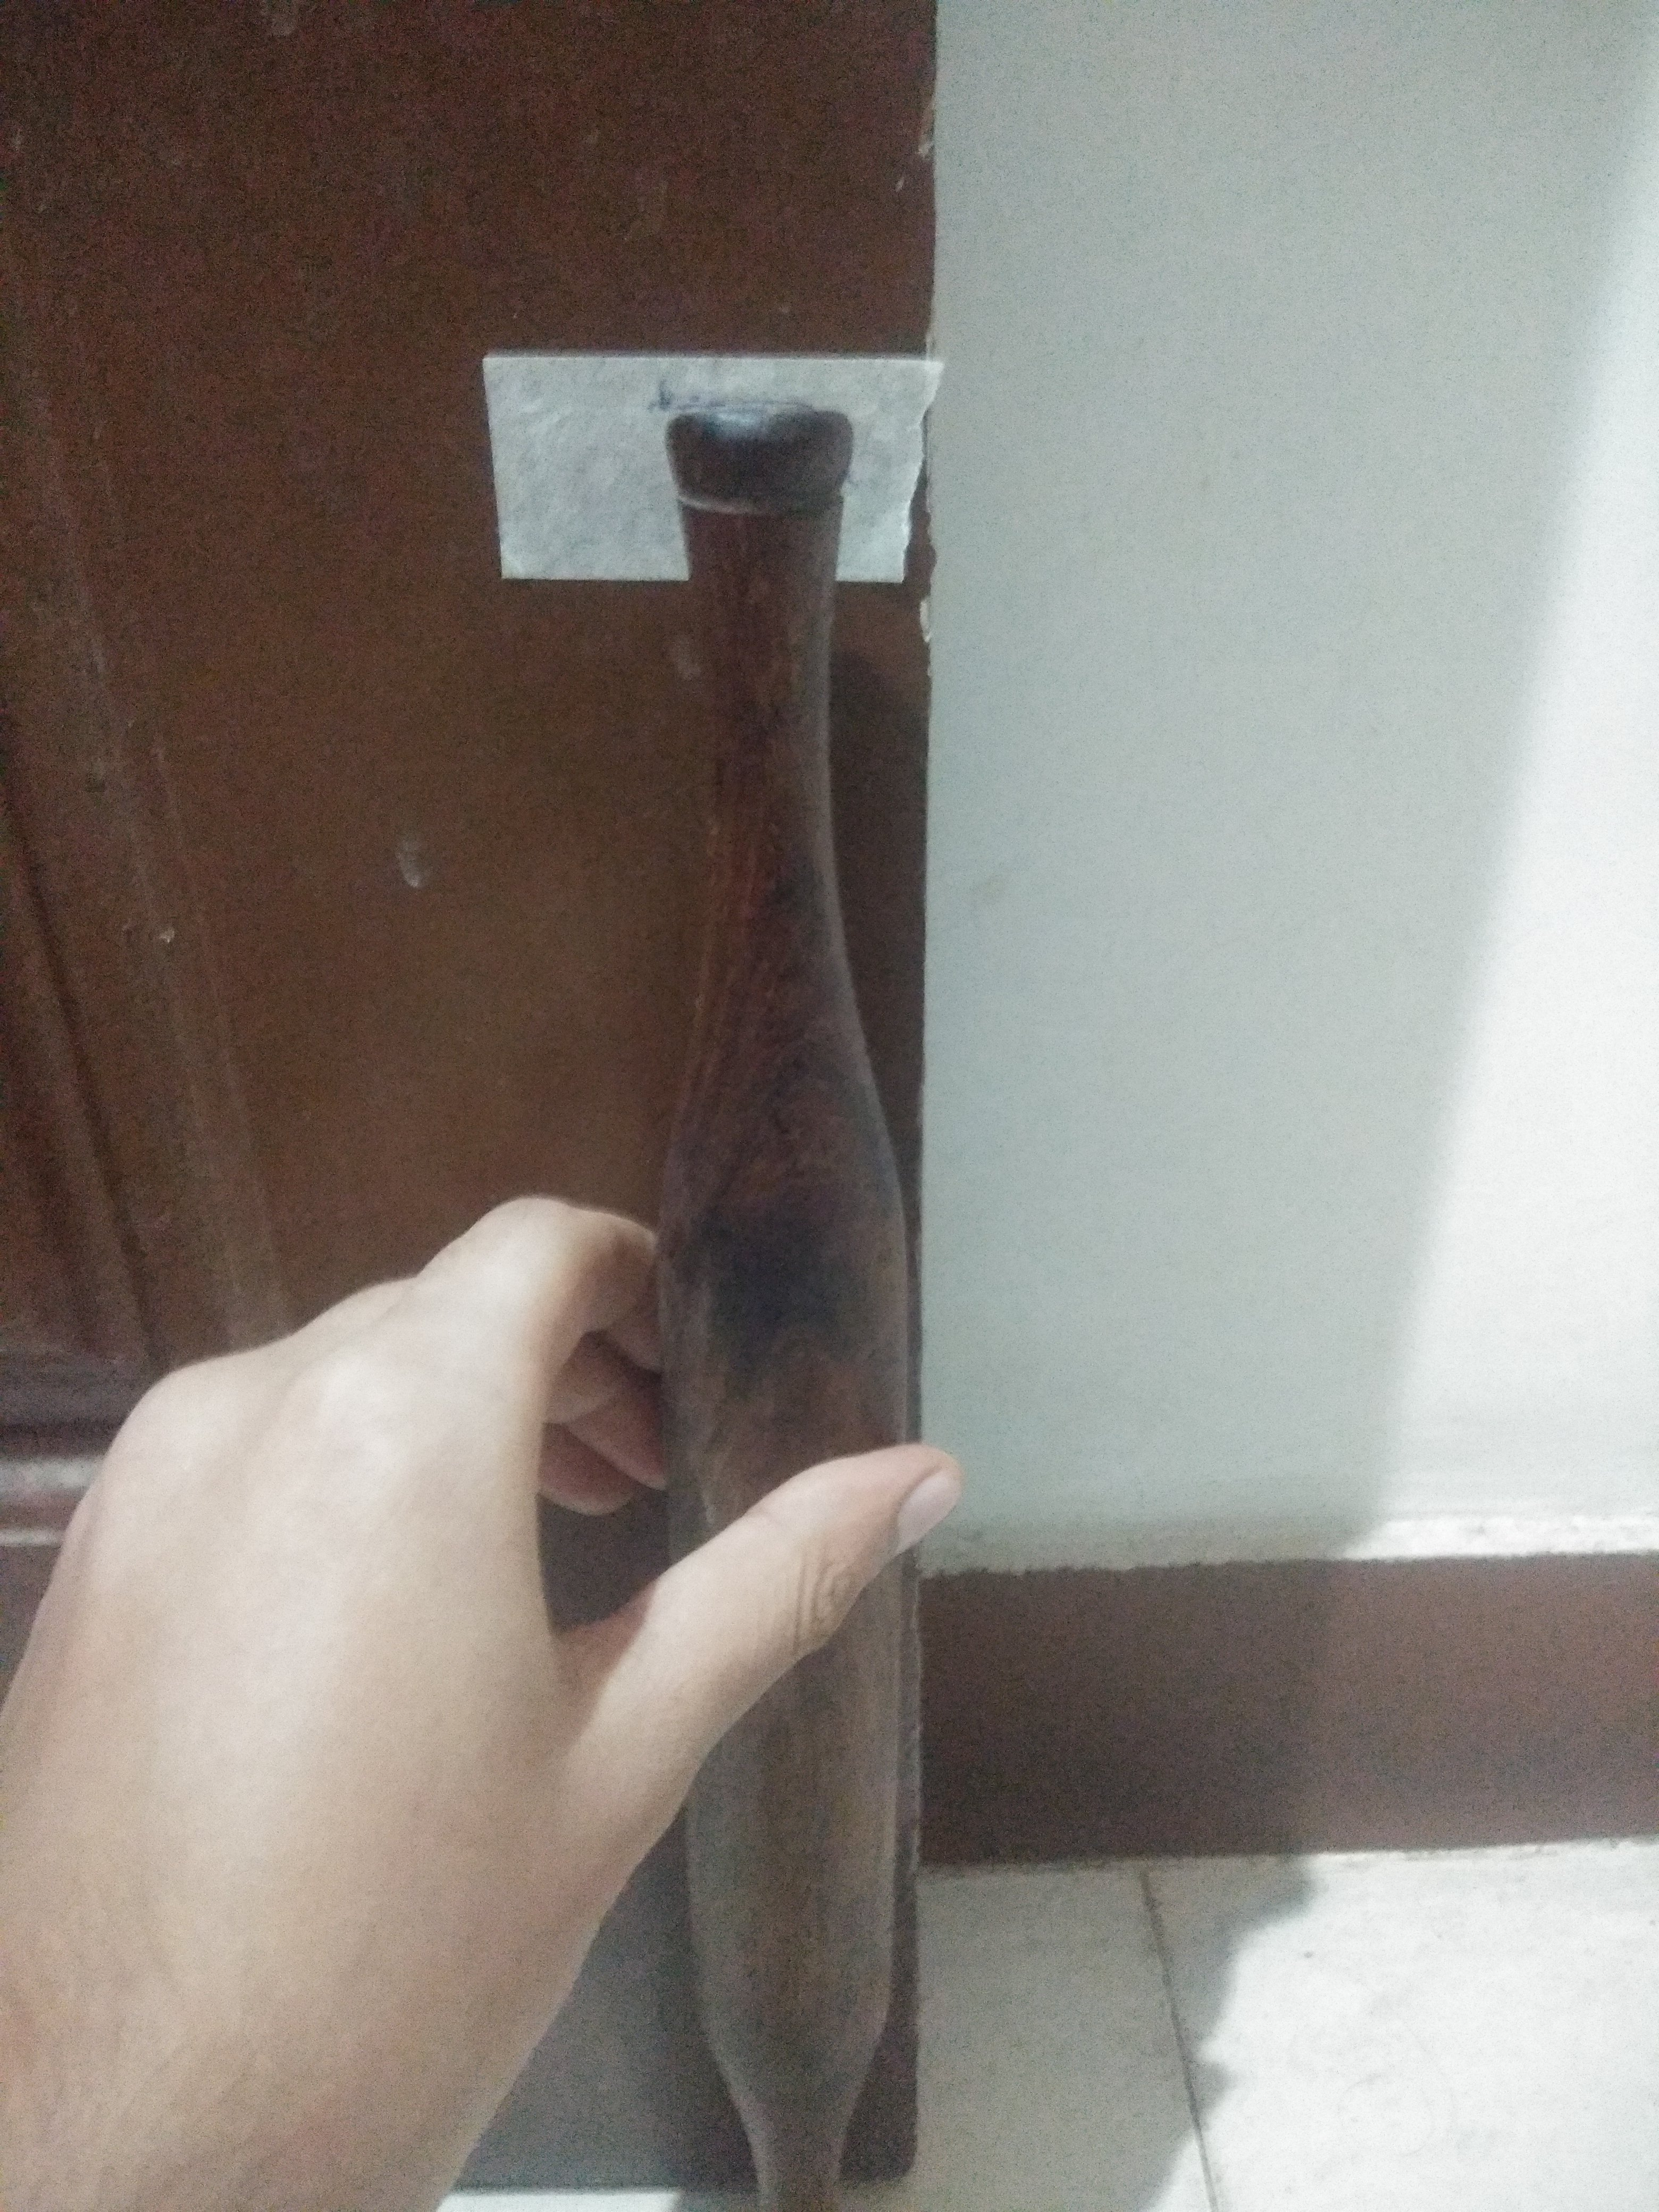
\includegraphics[width=0.4\paperwidth]{Videos/belanHeght1}

\caption{Measurement of length of belan\label{fig:BelanLegth1}}
\end{figure}

\begin{figure}[H]
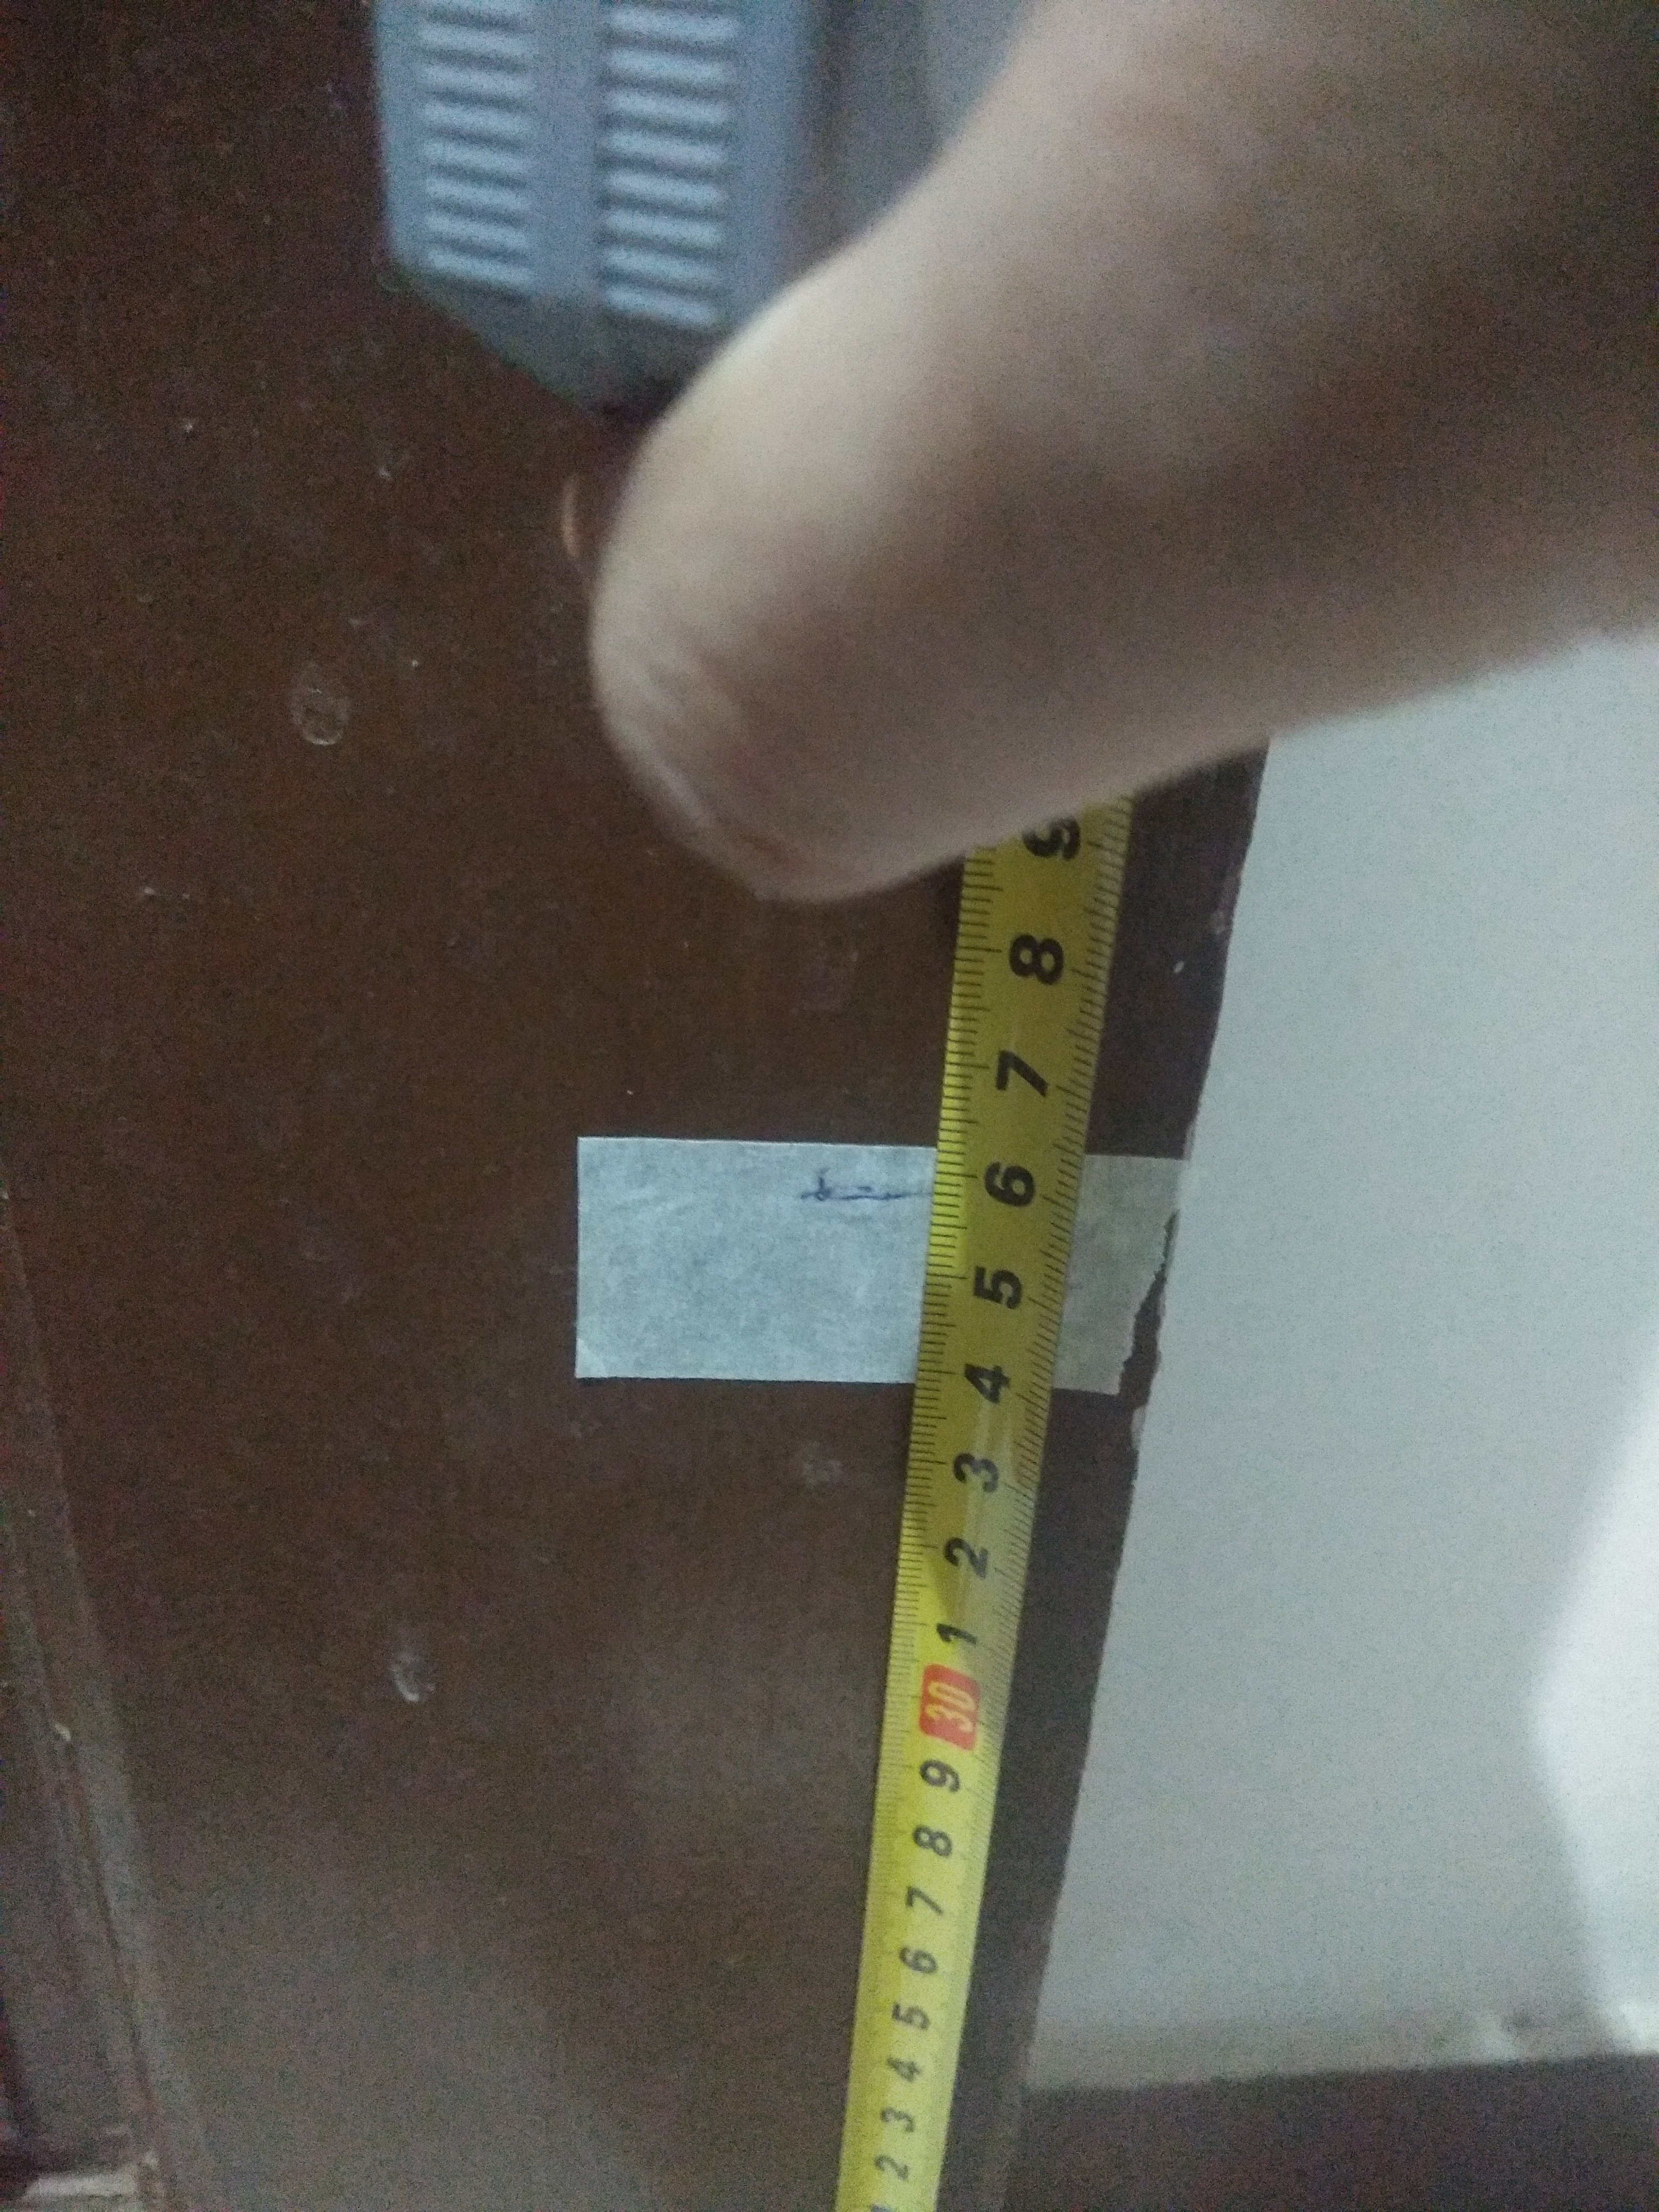
\includegraphics[width=0.4\paperwidth]{Videos/belanHeght2}

\caption{Measurement of length of belan\label{fig:BelanLegth2}}
\end{figure}


\subsubsection{Measurement of distance travelled by belan}

The bench used for the experiment has total length as 172cm (fig \ref{fig:Belan Length}
). However the belan can travel only part of the distance. On either
side, the shape of the belan prevents it from starting at the very
end (and reaching the lowest point) thus a tape has been put to keep
track of the start and the end point of the belan. As seen from the
Figure \ref{fig:Belan Length-left} \& \ref{fig:Belan Length-right}
, the total length the belan can traverse is (166 - 4.3) = 161.7 cm.
The least count of the scale used here is 1mm. Therefore the total
length the belan can traverse is 161.7$\pm$ 0.1 cm.

\begin{figure}[H]
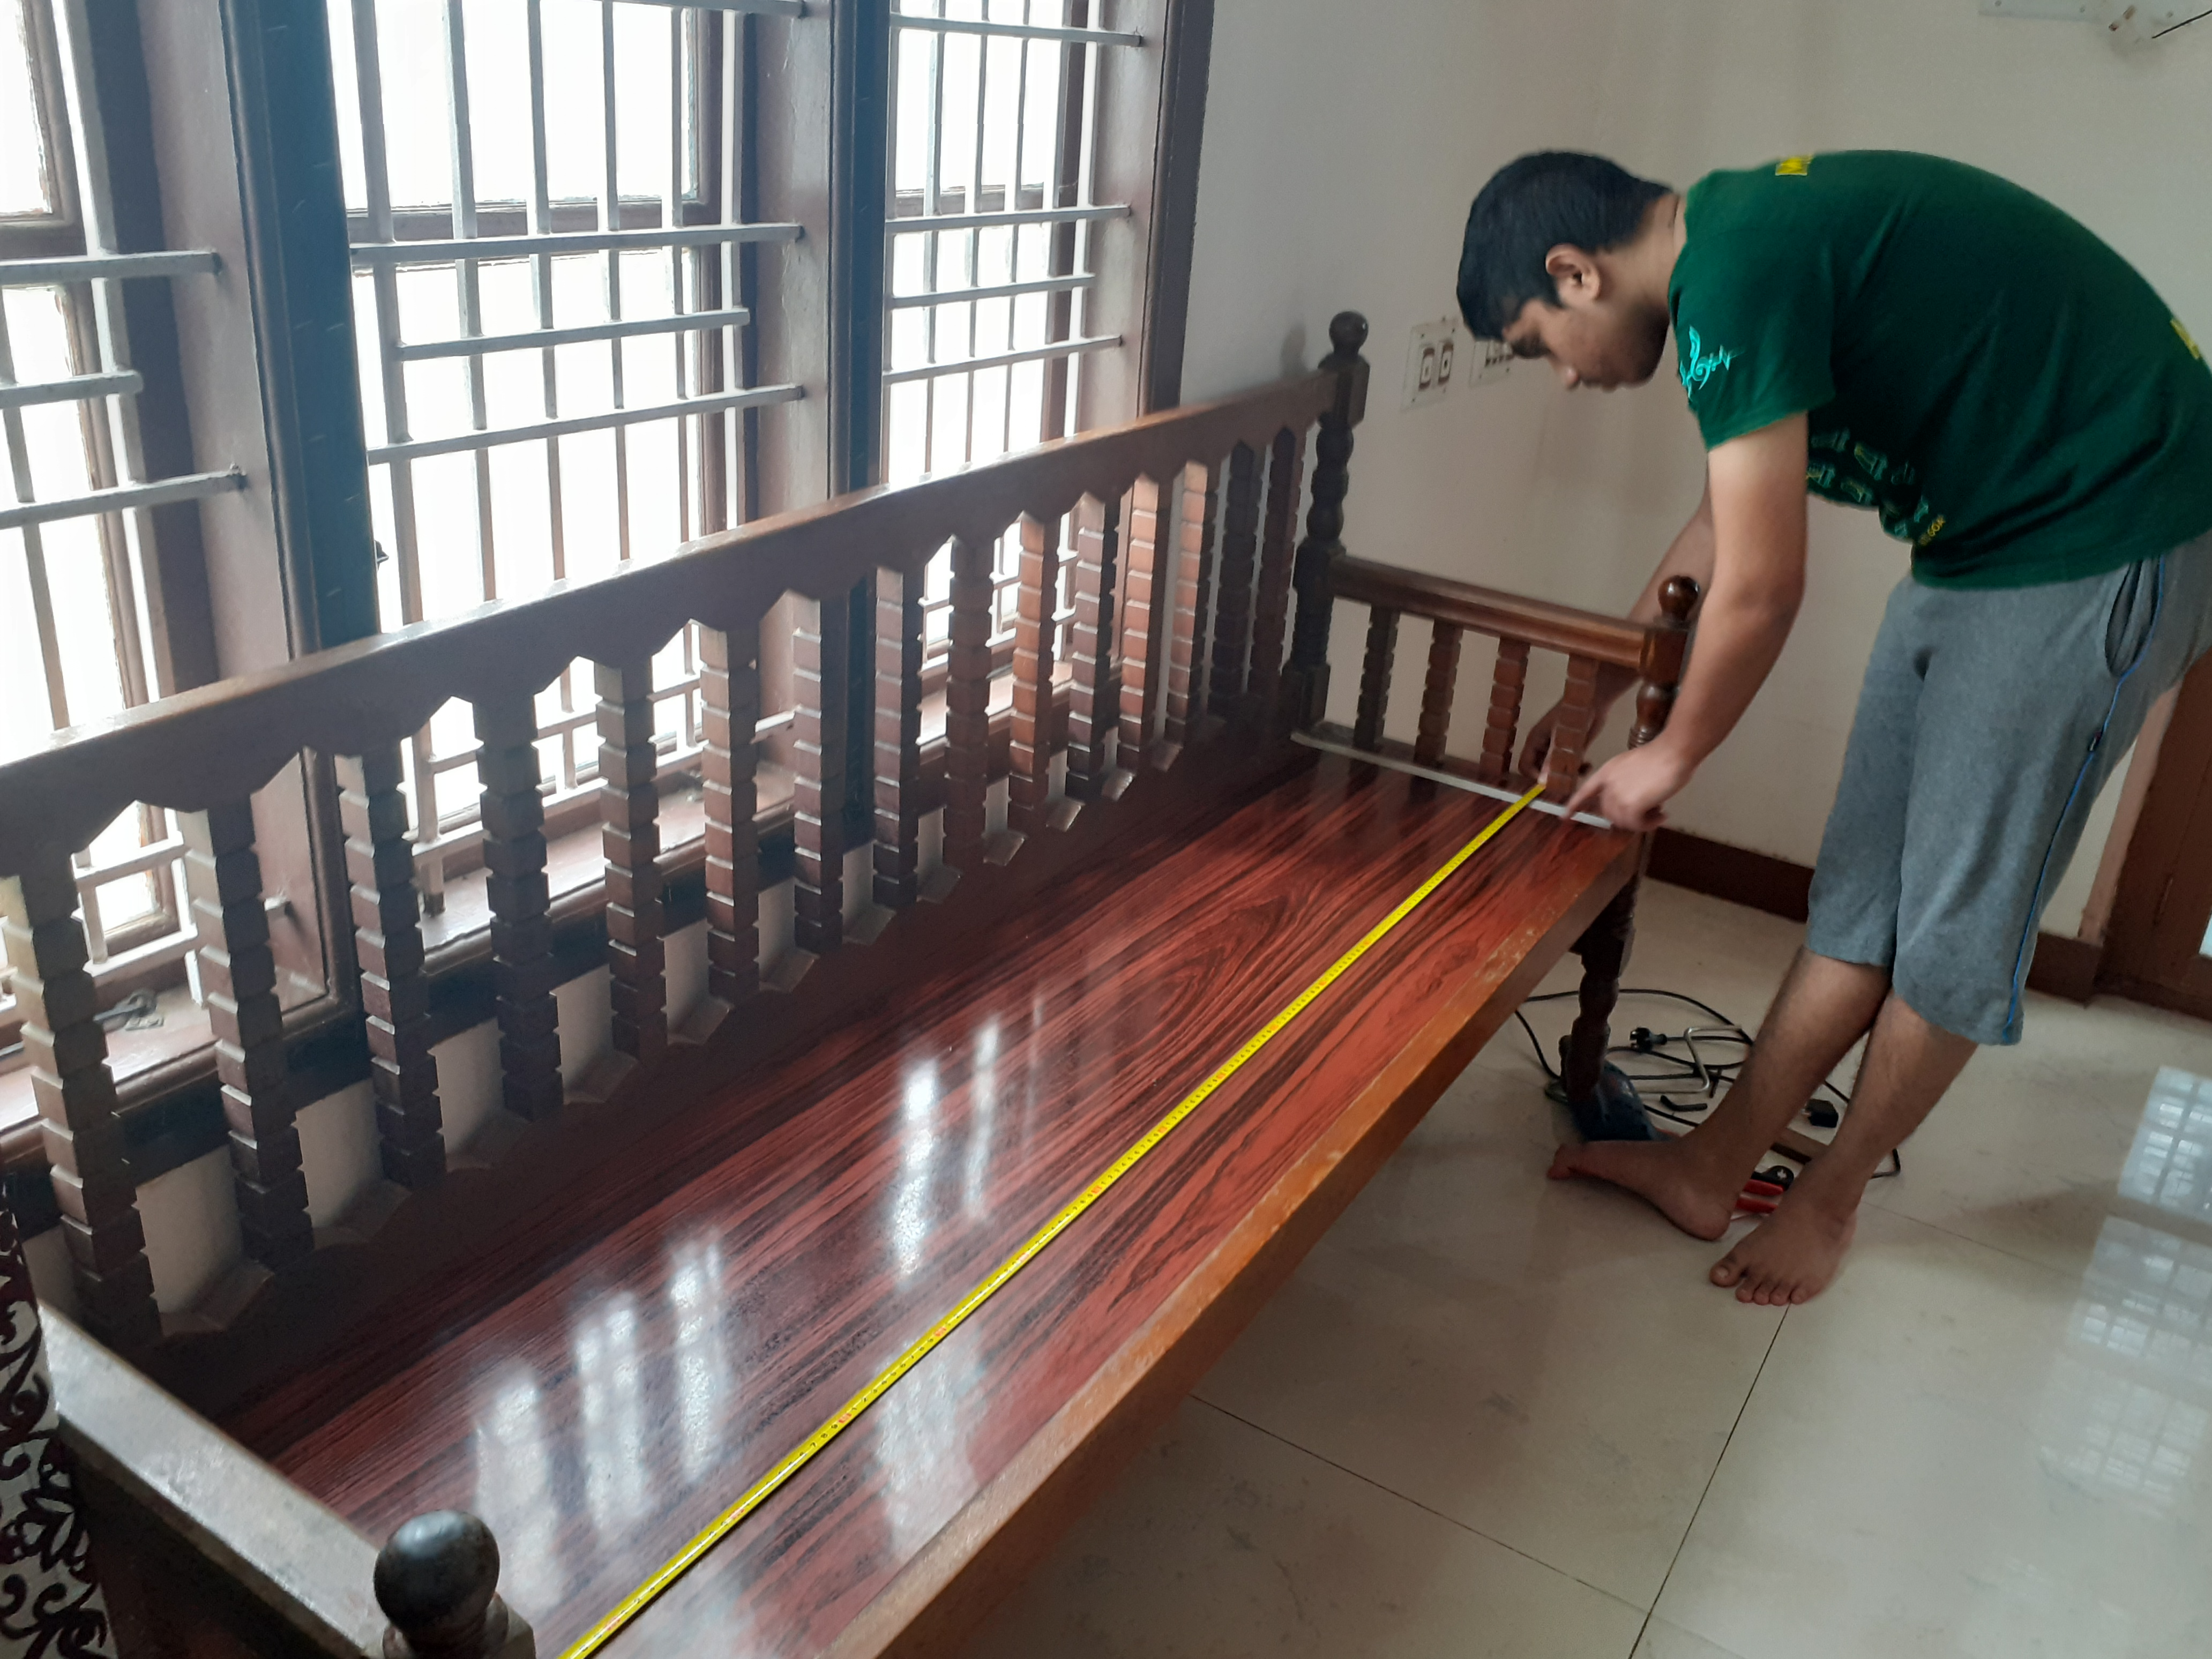
\includegraphics[width=0.4\paperwidth]{Videos/measure_table_lenght}

\caption{Measurement of distance travelled by belan\label{fig:Belan Length}}
\end{figure}

\begin{figure}[H]
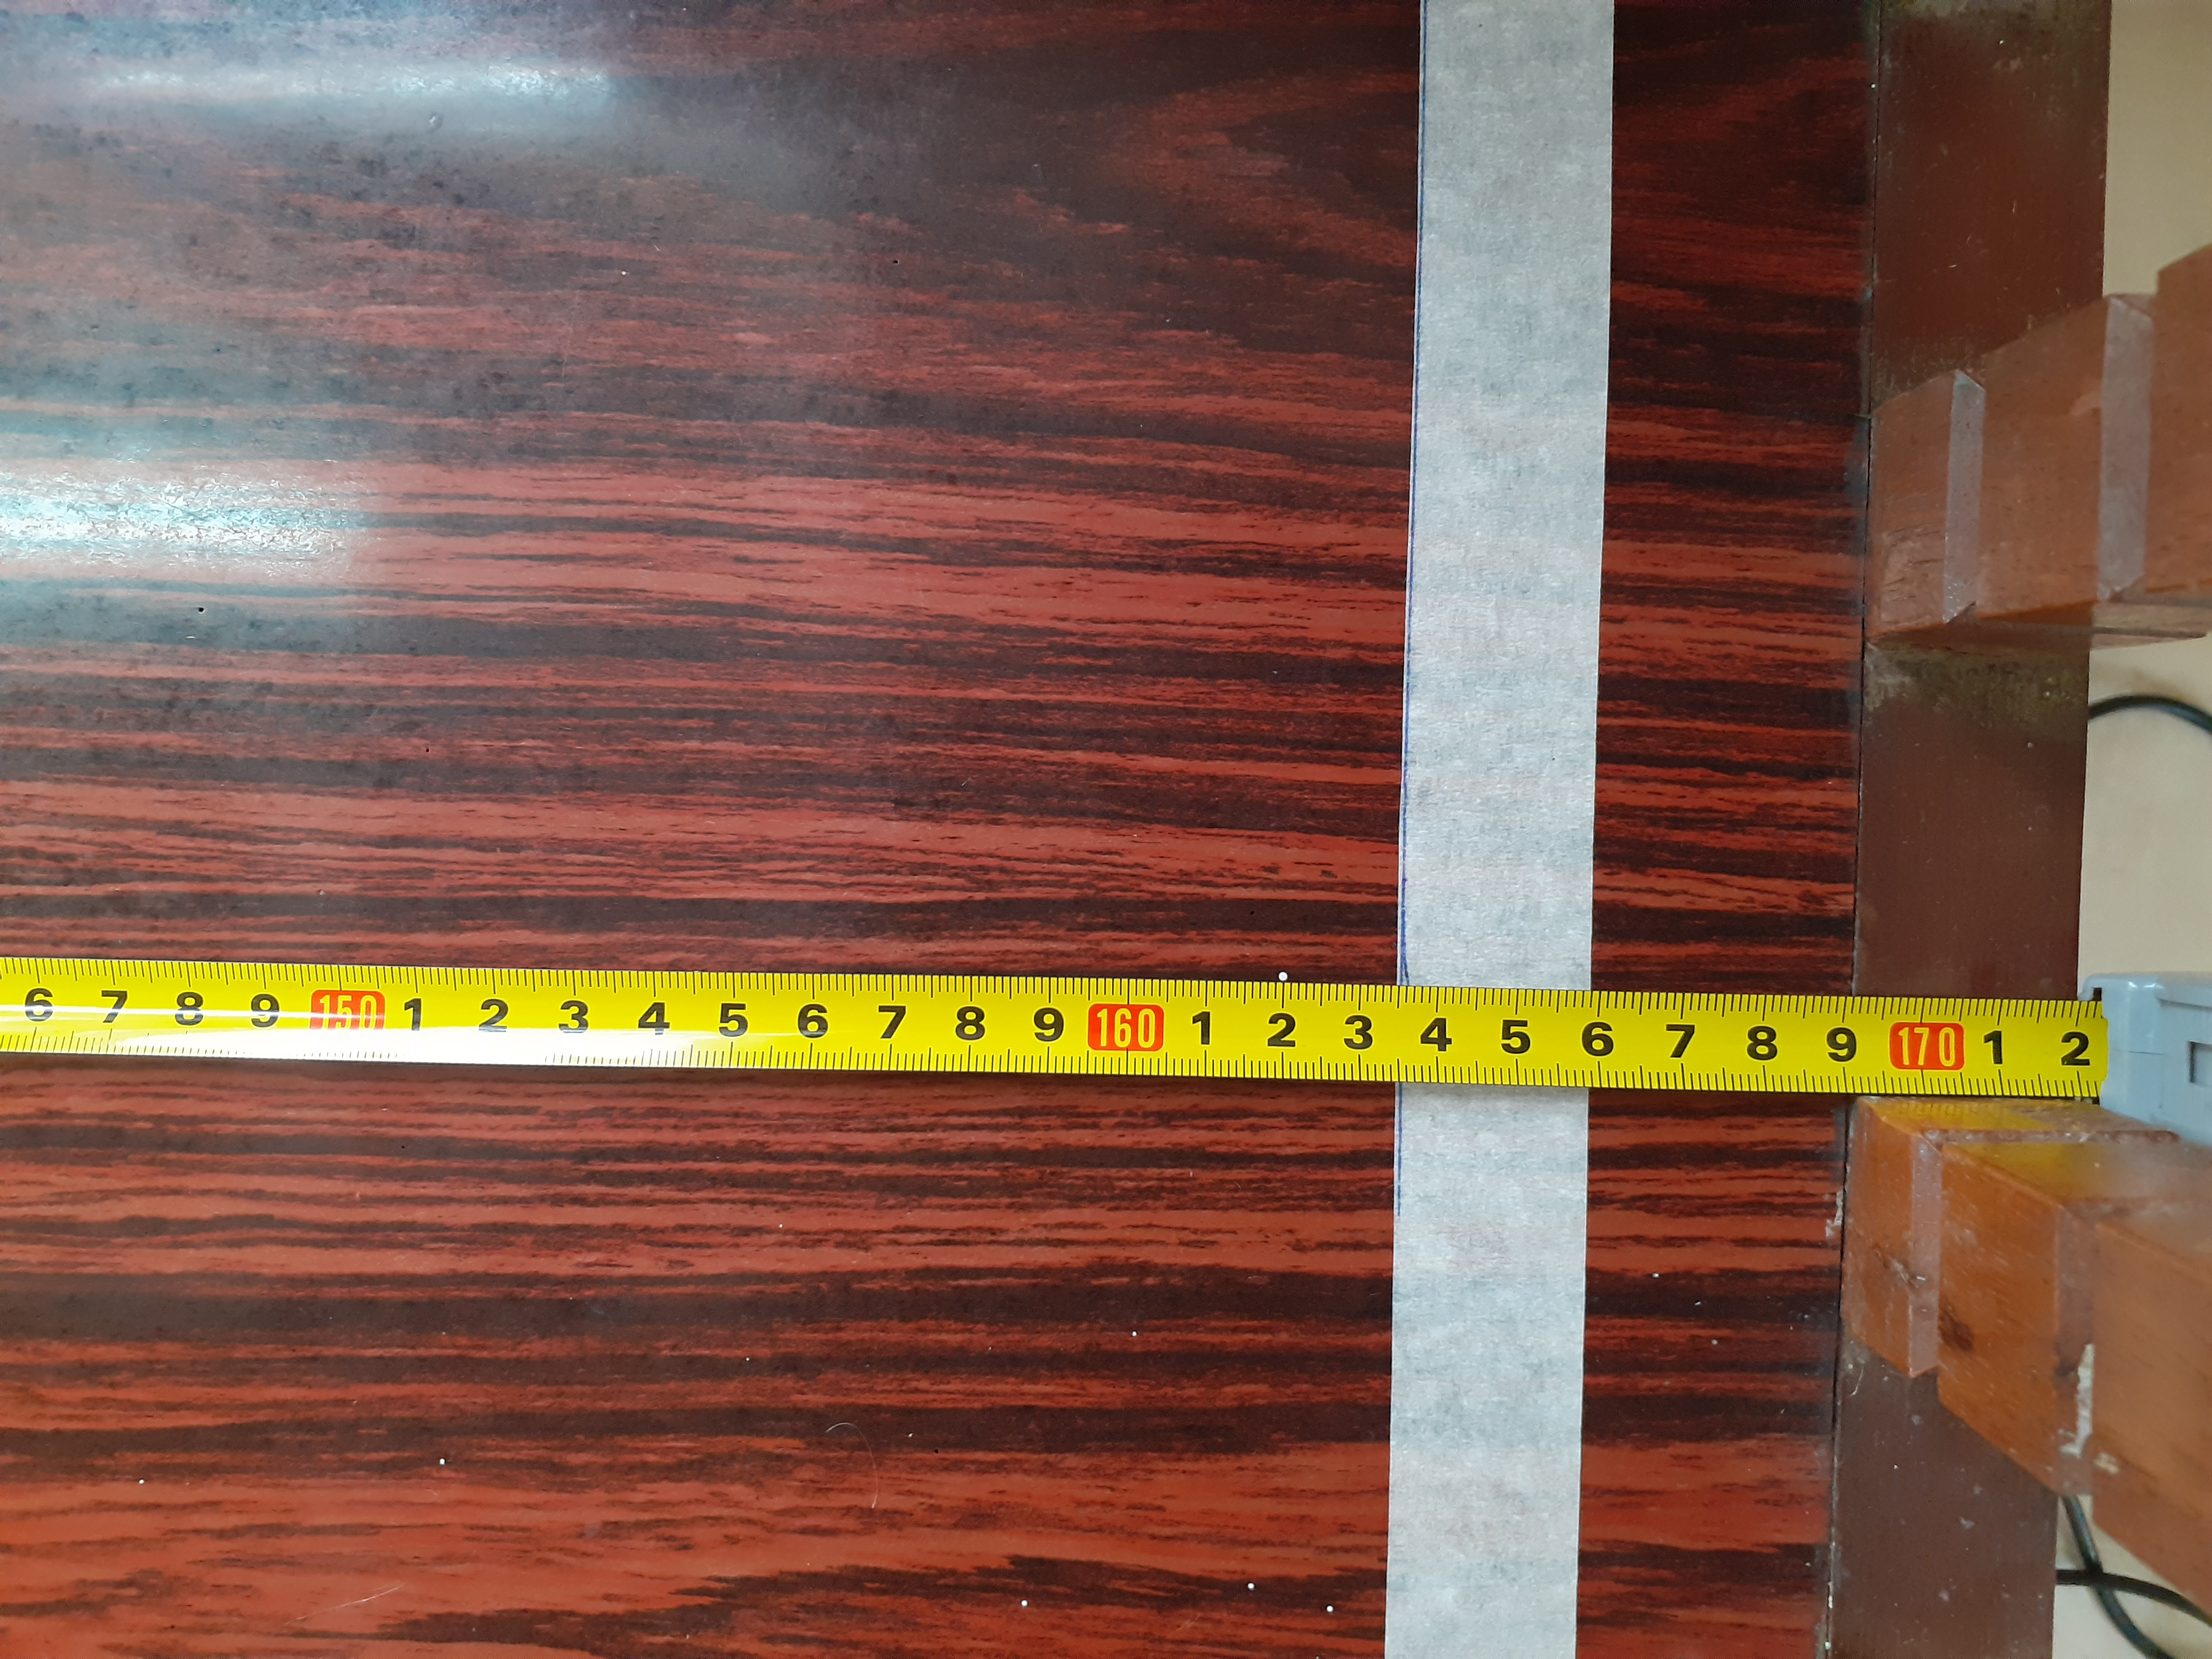
\includegraphics[width=0.4\paperwidth]{Videos/measure_right_lenght}

\caption{Measurement of distance travelled by belan (right end)\label{fig:Belan Length-right}}
\end{figure}

\begin{figure}[H]
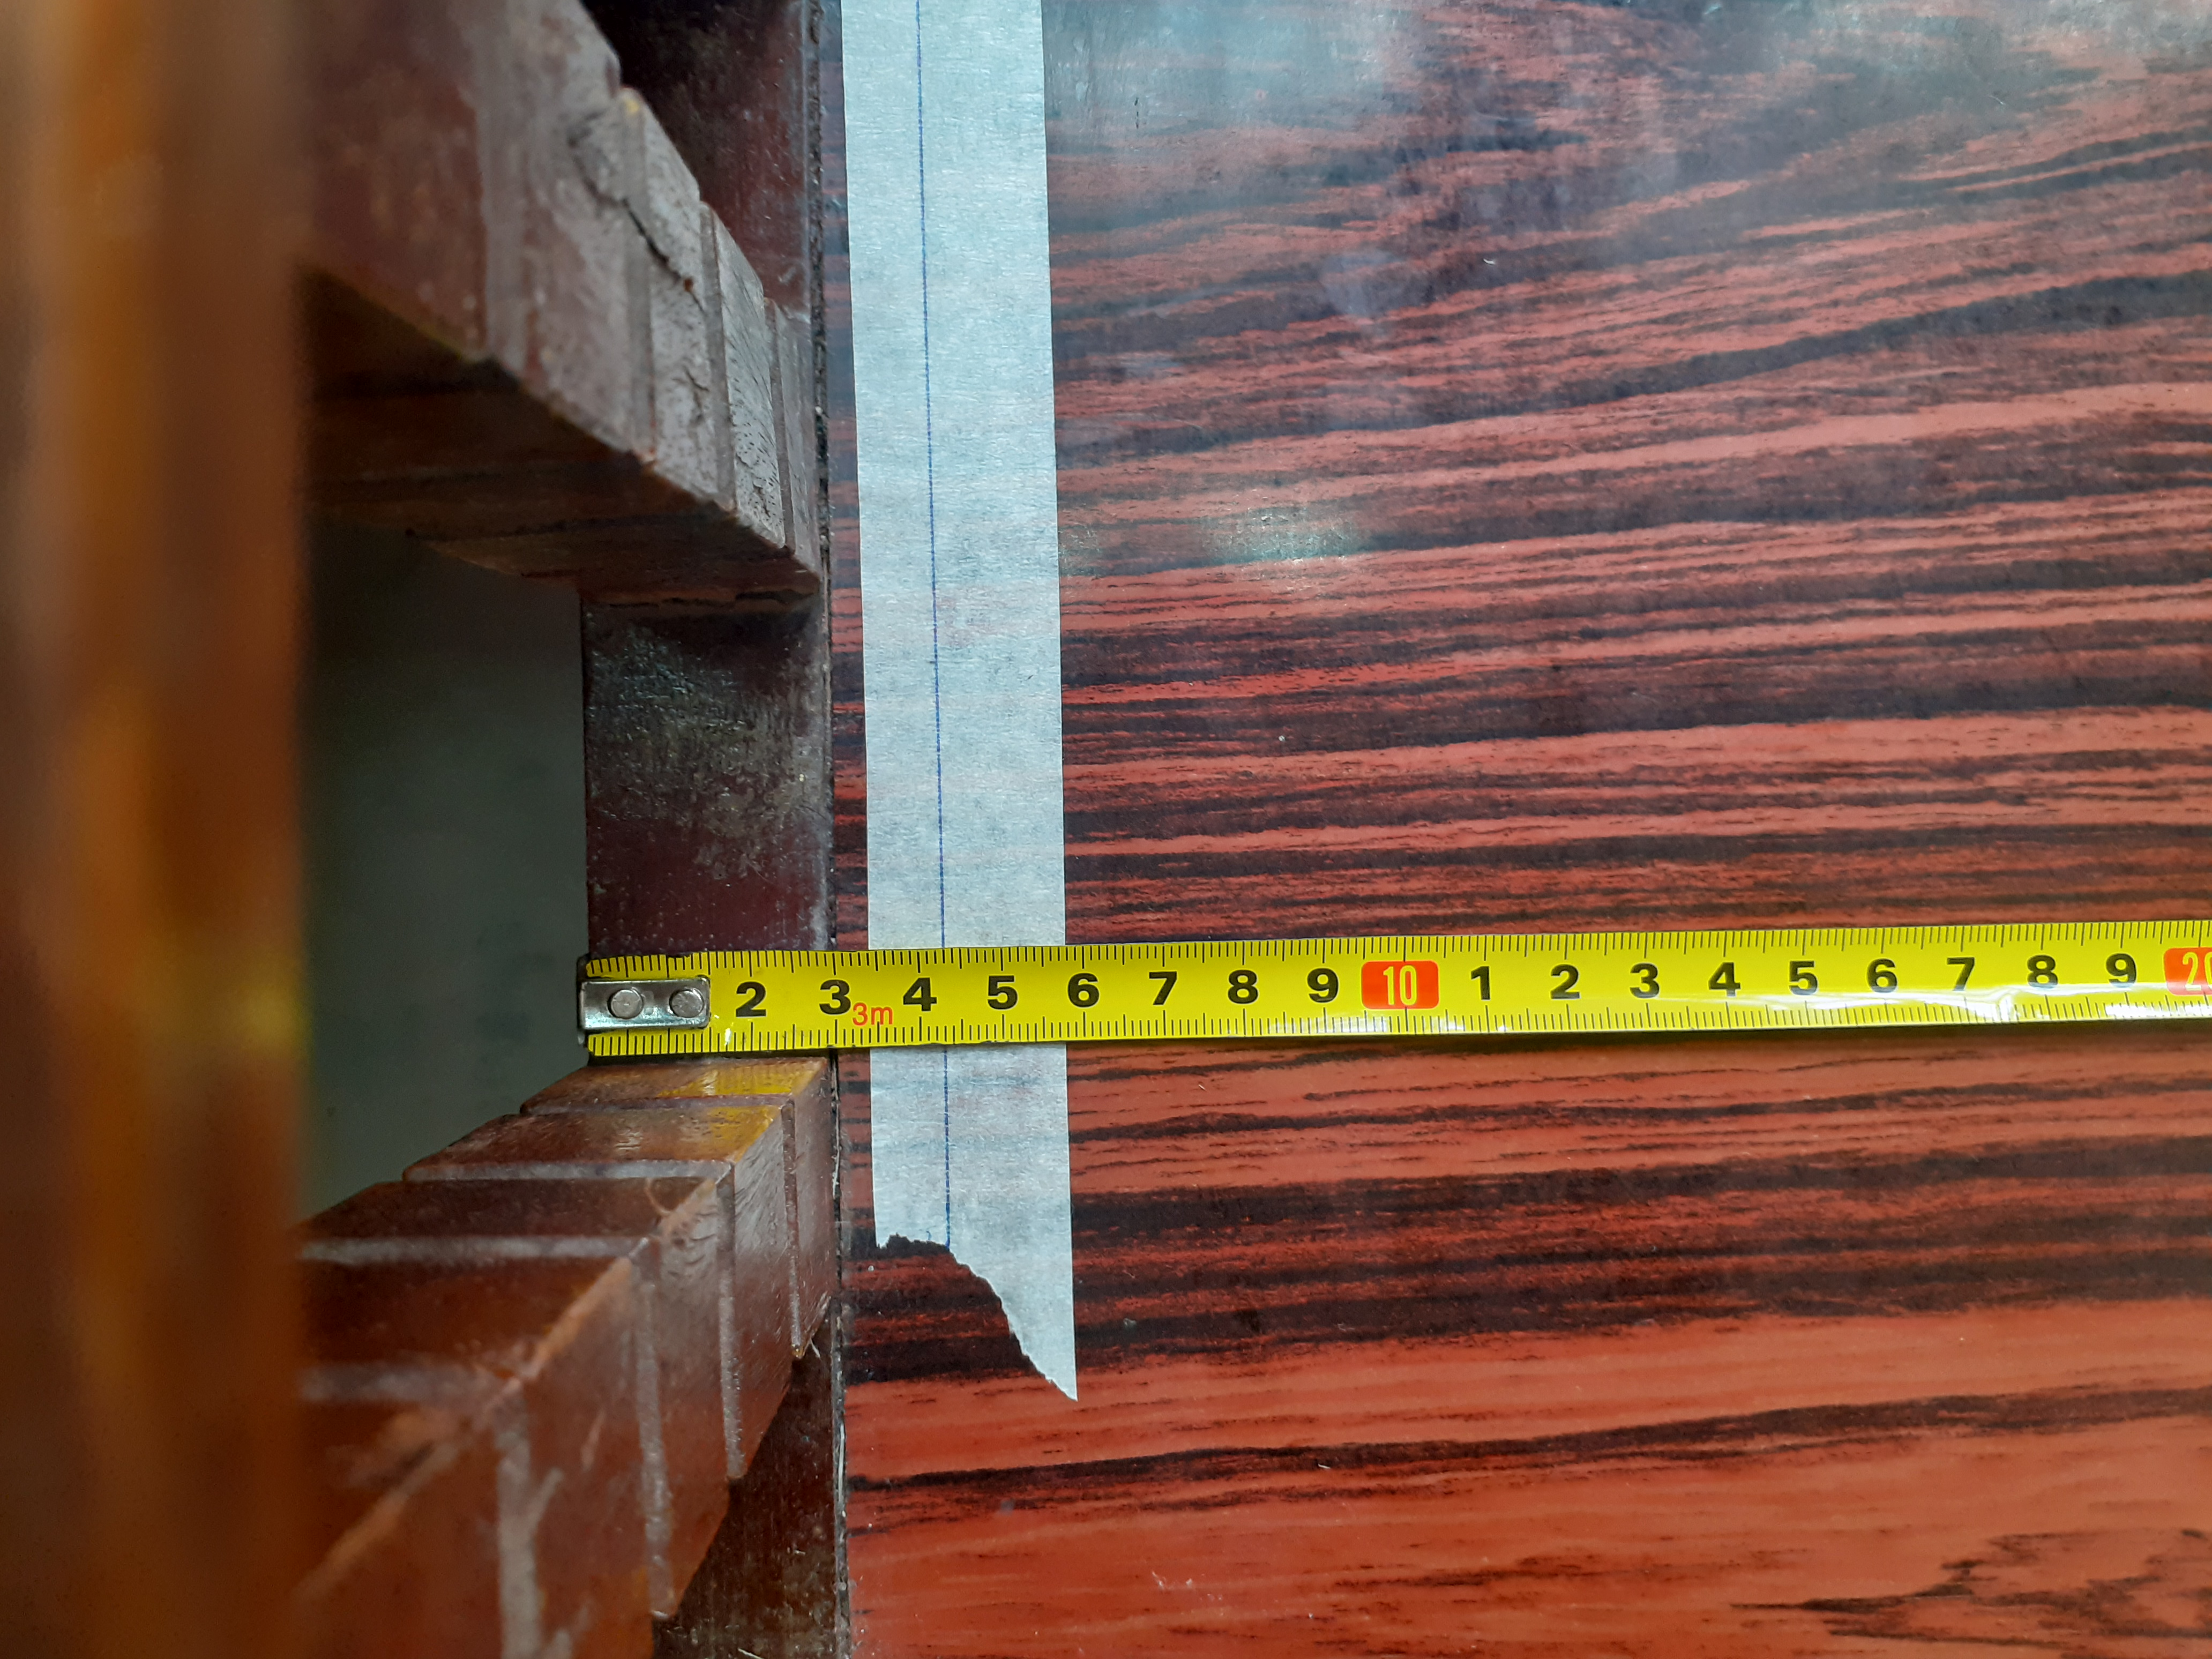
\includegraphics[width=0.4\paperwidth]{Videos/measure_left_lenght}

\caption{Measurement of distance travelled by belan (right end)\label{fig:Belan Length-left}}
\end{figure}


\subsubsection{Measurement of vertical lift at one end}

The selected bench for measurement has maximum flat length as 172
cm. We want to perform experiment at angles from 2 degree to 16 degree
at an interval of 2. We can calculate the height required to be lifted
at one end to reach the given set of angles as $L=172\sin\theta$.
This gives us the following table \ref{tab:Measurement-of-vertical}
.

\begin{table}[H]
\begin{tabular}{|l|l|l|}
\hline 
Angle(degree) & lift required (cm) & lift rounded to LC of scale (cm)\tabularnewline
\hline 
2 & 6.003 & 6\tabularnewline
\hline 
4 & 11.998 & 12\tabularnewline
\hline 
6 & 17.979 & 18\tabularnewline
\hline 
8 & 23.938 & 24\tabularnewline
\hline 
10 & 29.867 & 30\tabularnewline
\hline 
12 & 35.761 & 35.8\tabularnewline
\hline 
14 & 41.611 & 41.6\tabularnewline
\hline 
16 & 47.410 & 47.4\tabularnewline
\hline 
\end{tabular}\caption{Measurement of vertical lift at one end \label{tab:Measurement-of-vertical}}
\end{table}
.

The Car Jack has been placed at the middle of one end of the bench
(Fig\ref{fig:Jack balance} ). For larger lengths (20cm onward) a
set of wooden planks are added to increase the height (Fig \ref{fig:Jack wood}).
The bench can be lifted higher by rotating the shaft of the car jack
until the required height is met (Fig ). Since the height can be measured
to 0.1cm accuracy (LC of the scale used) this also translates into
the accuracy for angle of the inclined plane. While measuring height
care must be taken that the scale is perpendicular to ground and the
height of the center of the bench leg is measured. One can use a flat
card as a pointer and to avoid parallax. (Fig \ref{fig:Jack measure})

\begin{figure}[H]
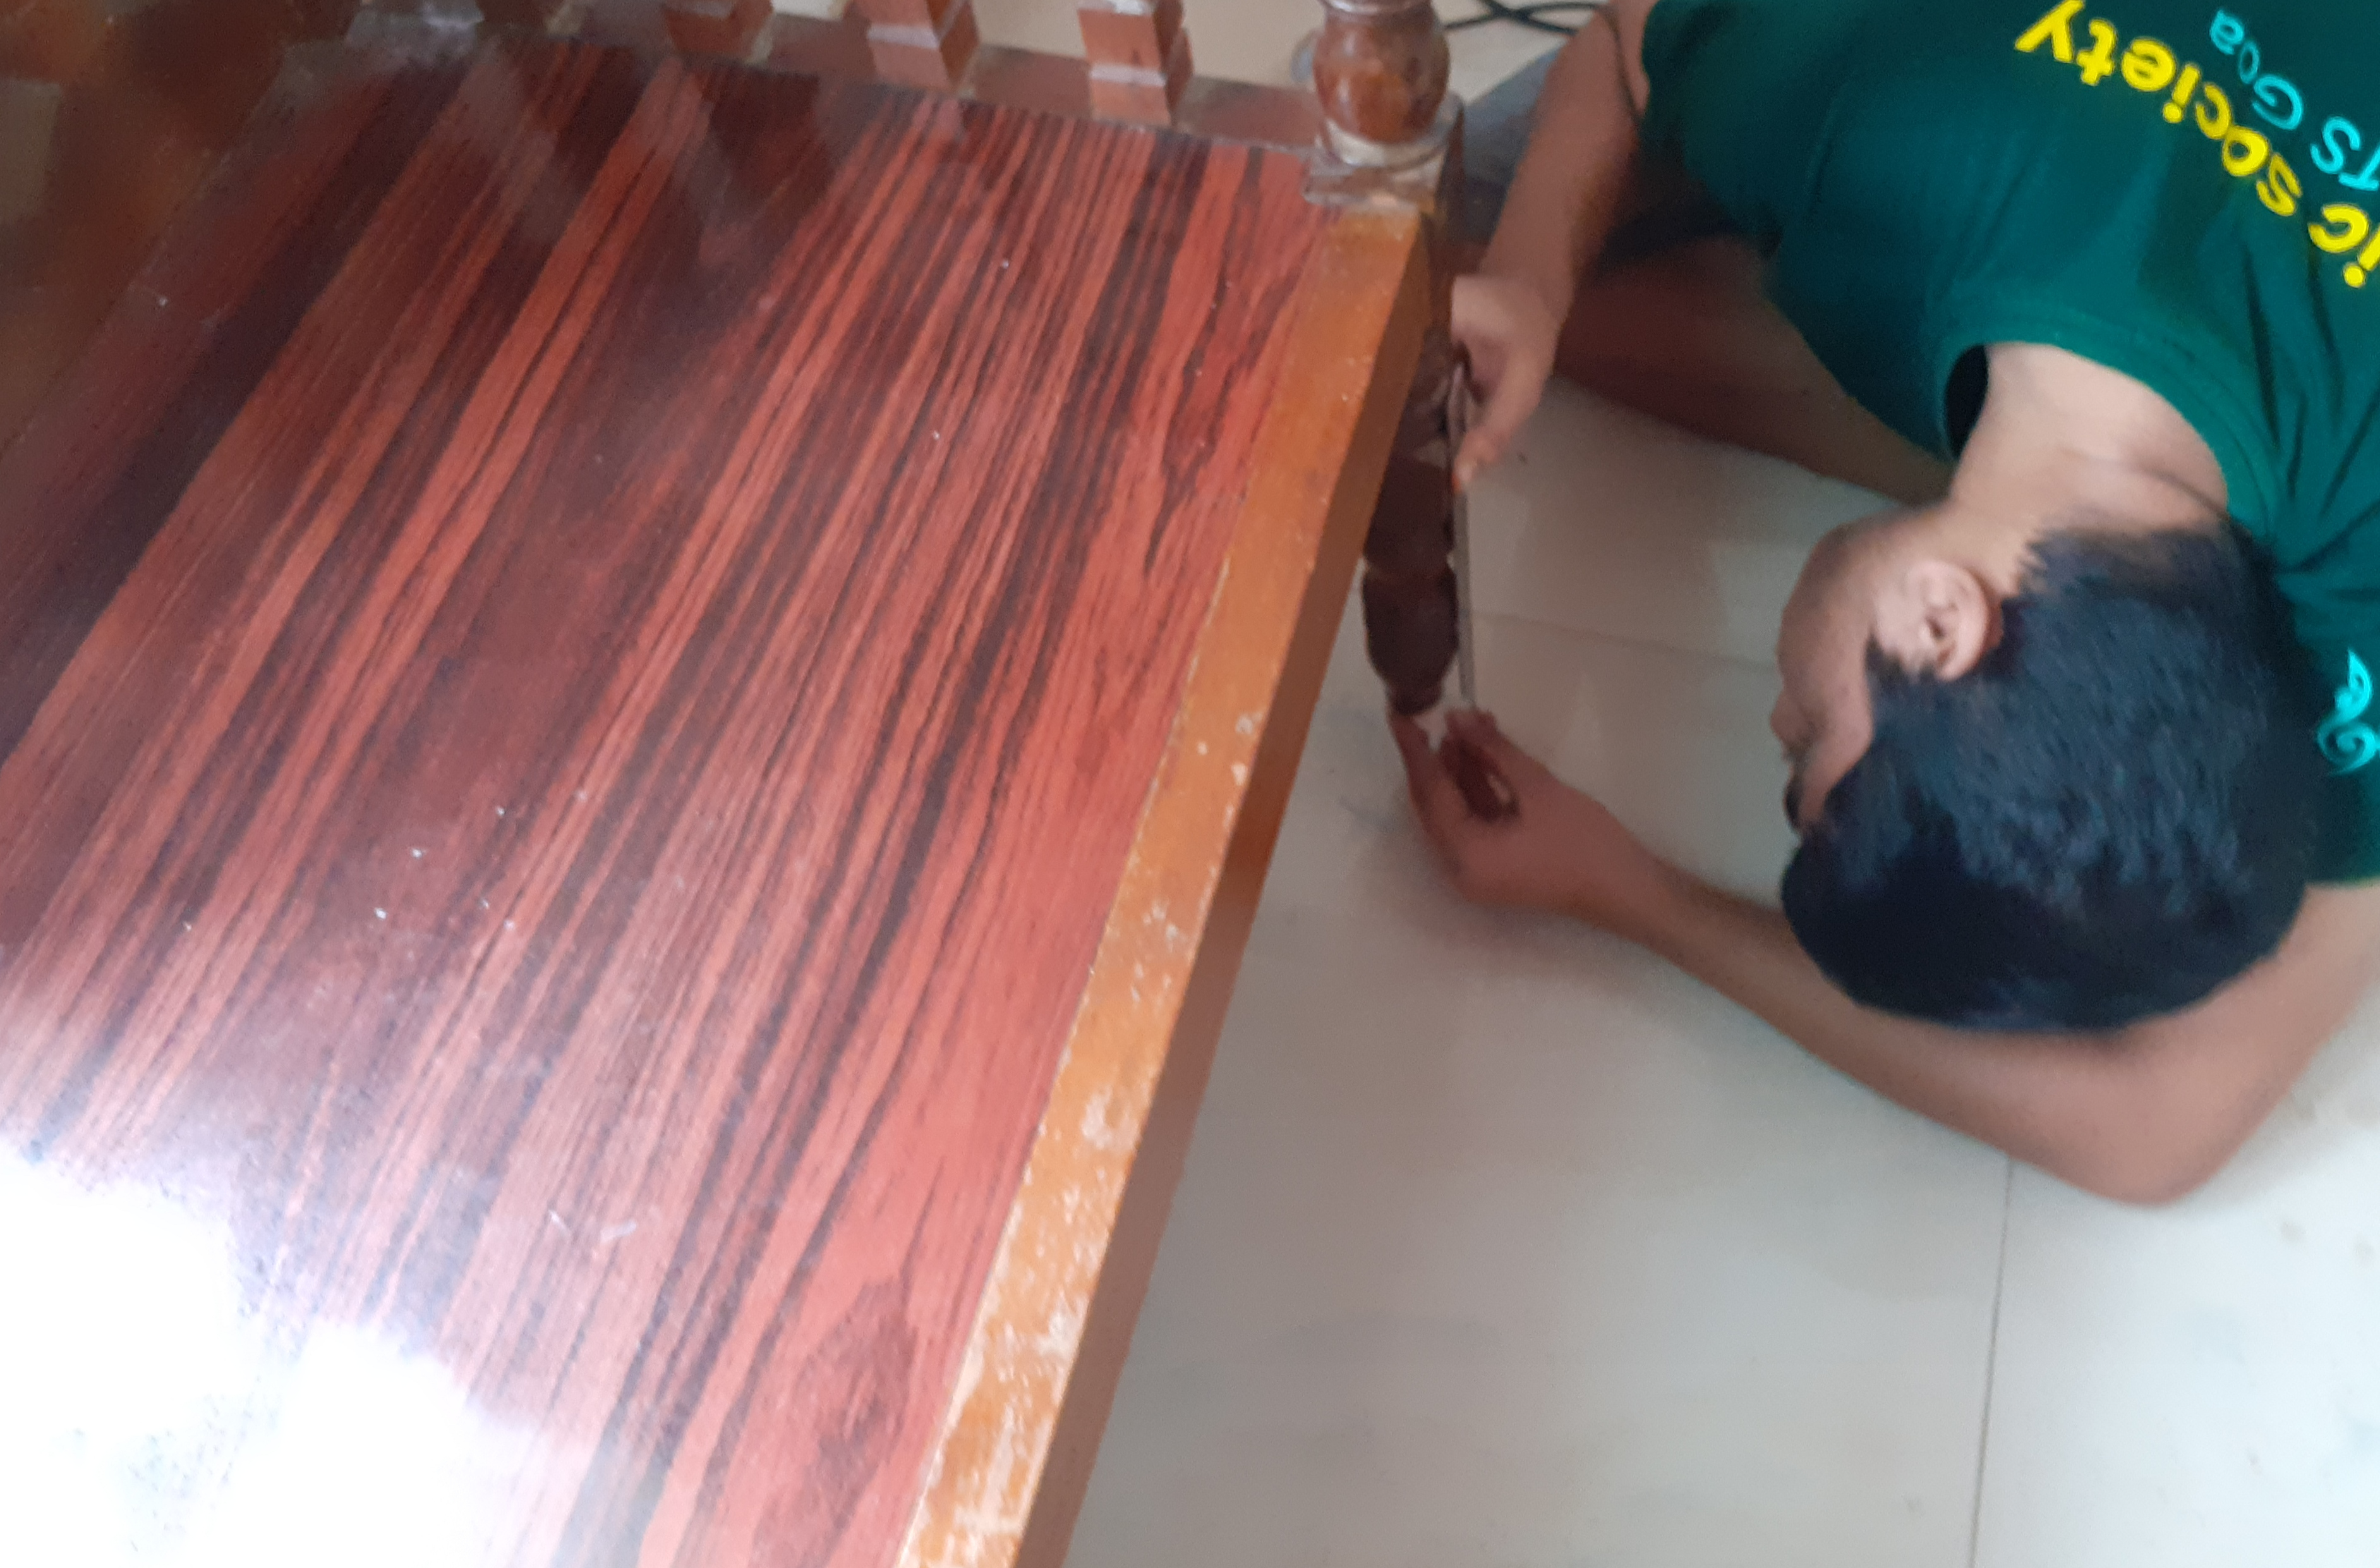
\includegraphics[width=0.4\paperwidth]{Videos/measureJack}

\caption{Measurement of vertical lift using scale and flat card.\label{fig:Jack measure}}
\end{figure}

\begin{figure}[H]
\includegraphics[width=0.4\paperwidth]{\string"Videos/jack on the bench\string".eps}

\caption{Placement of Car jack such that the bench is lifted and balanced.\label{fig:Jack balance}}
\end{figure}

\begin{figure}[H]
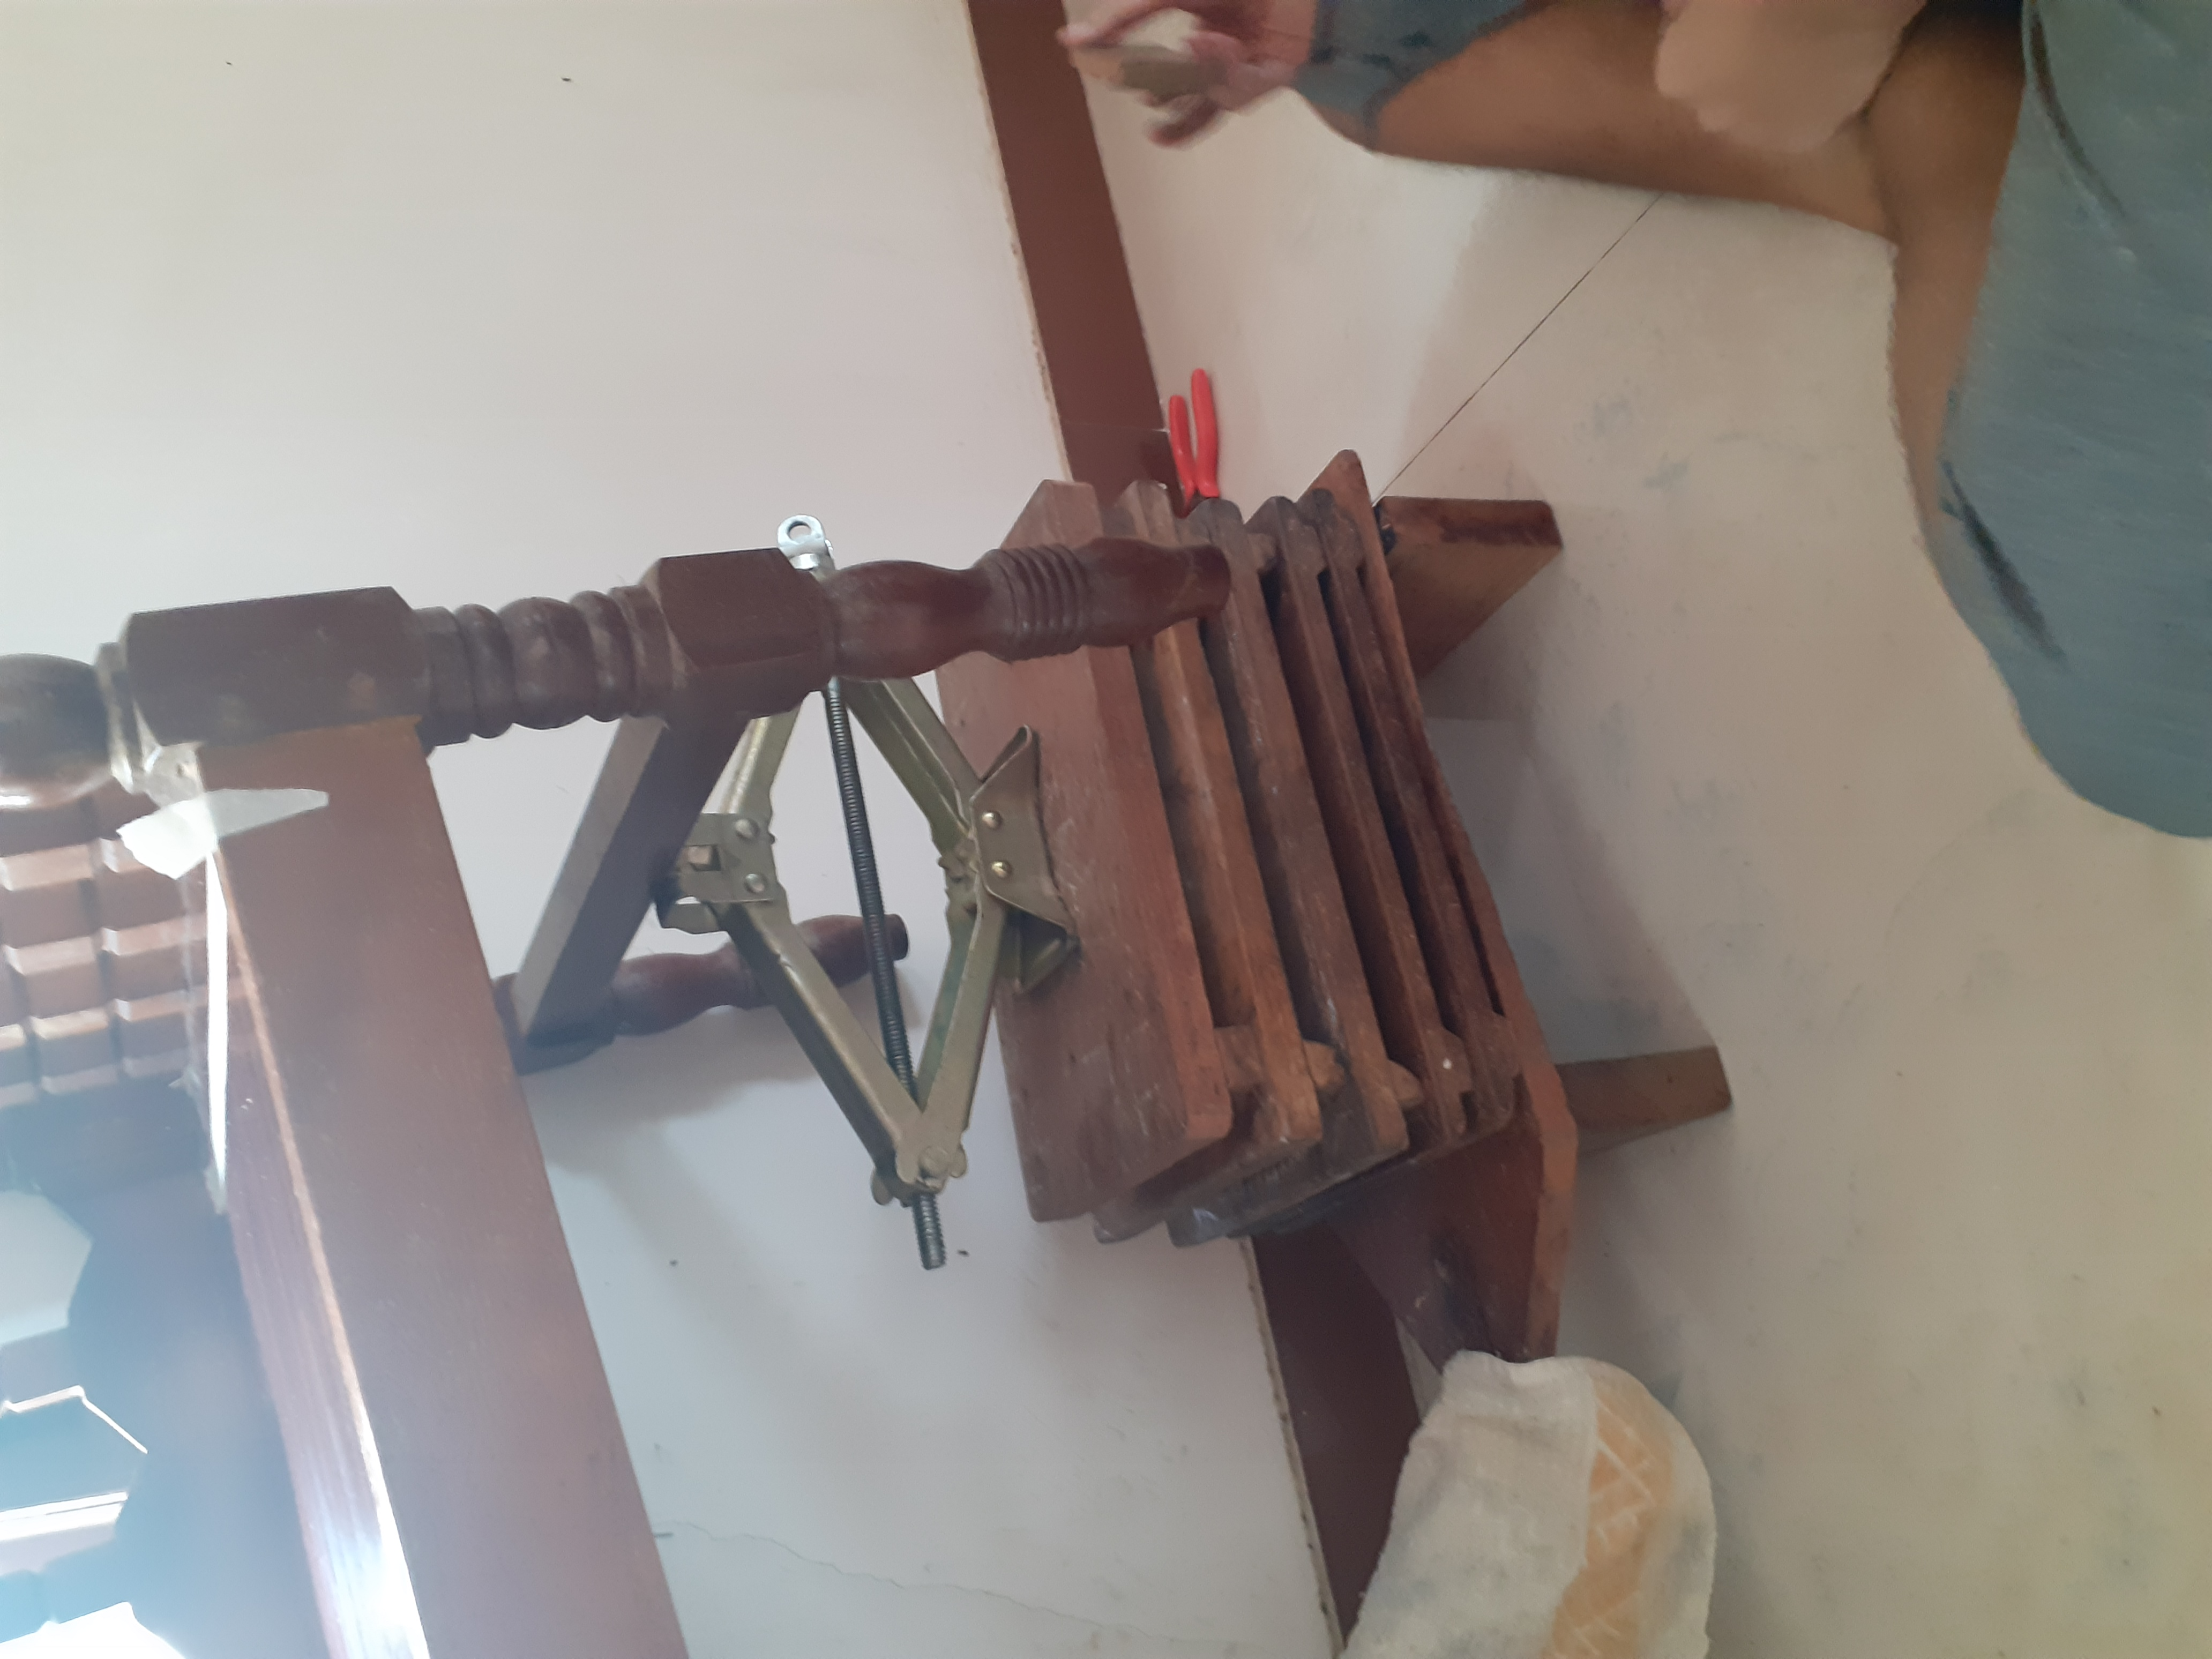
\includegraphics[width=0.4\paperwidth]{Videos/jack+ane2}

\caption{A set of wooden planks are added to increase the height.\label{fig:Jack wood}}
\end{figure}


\subsection{Measurement of time taken to roll down}

In order to measure the time taken for the belan to roll down, video
of the experiment was taken in a mobile phone. The video recorded
was then processed frame by frame to find the number of frames between
the starting and belan reaching the end. This analysis was done on
a mobile app named \textbf{``\href{https://play.google.com/store/apps/details?id=us.secondscount&hl=en_IN}{Video Stopwatch}''}
(As seen in fig \ref{fig:Screeenshot} ) .The video recorded had a
30 FPS (frames per second) thus each frame lasts for 33.33 ms and
this is our least count. This exercises was done 3 times and the average
was calculated.

\begin{figure}[H]
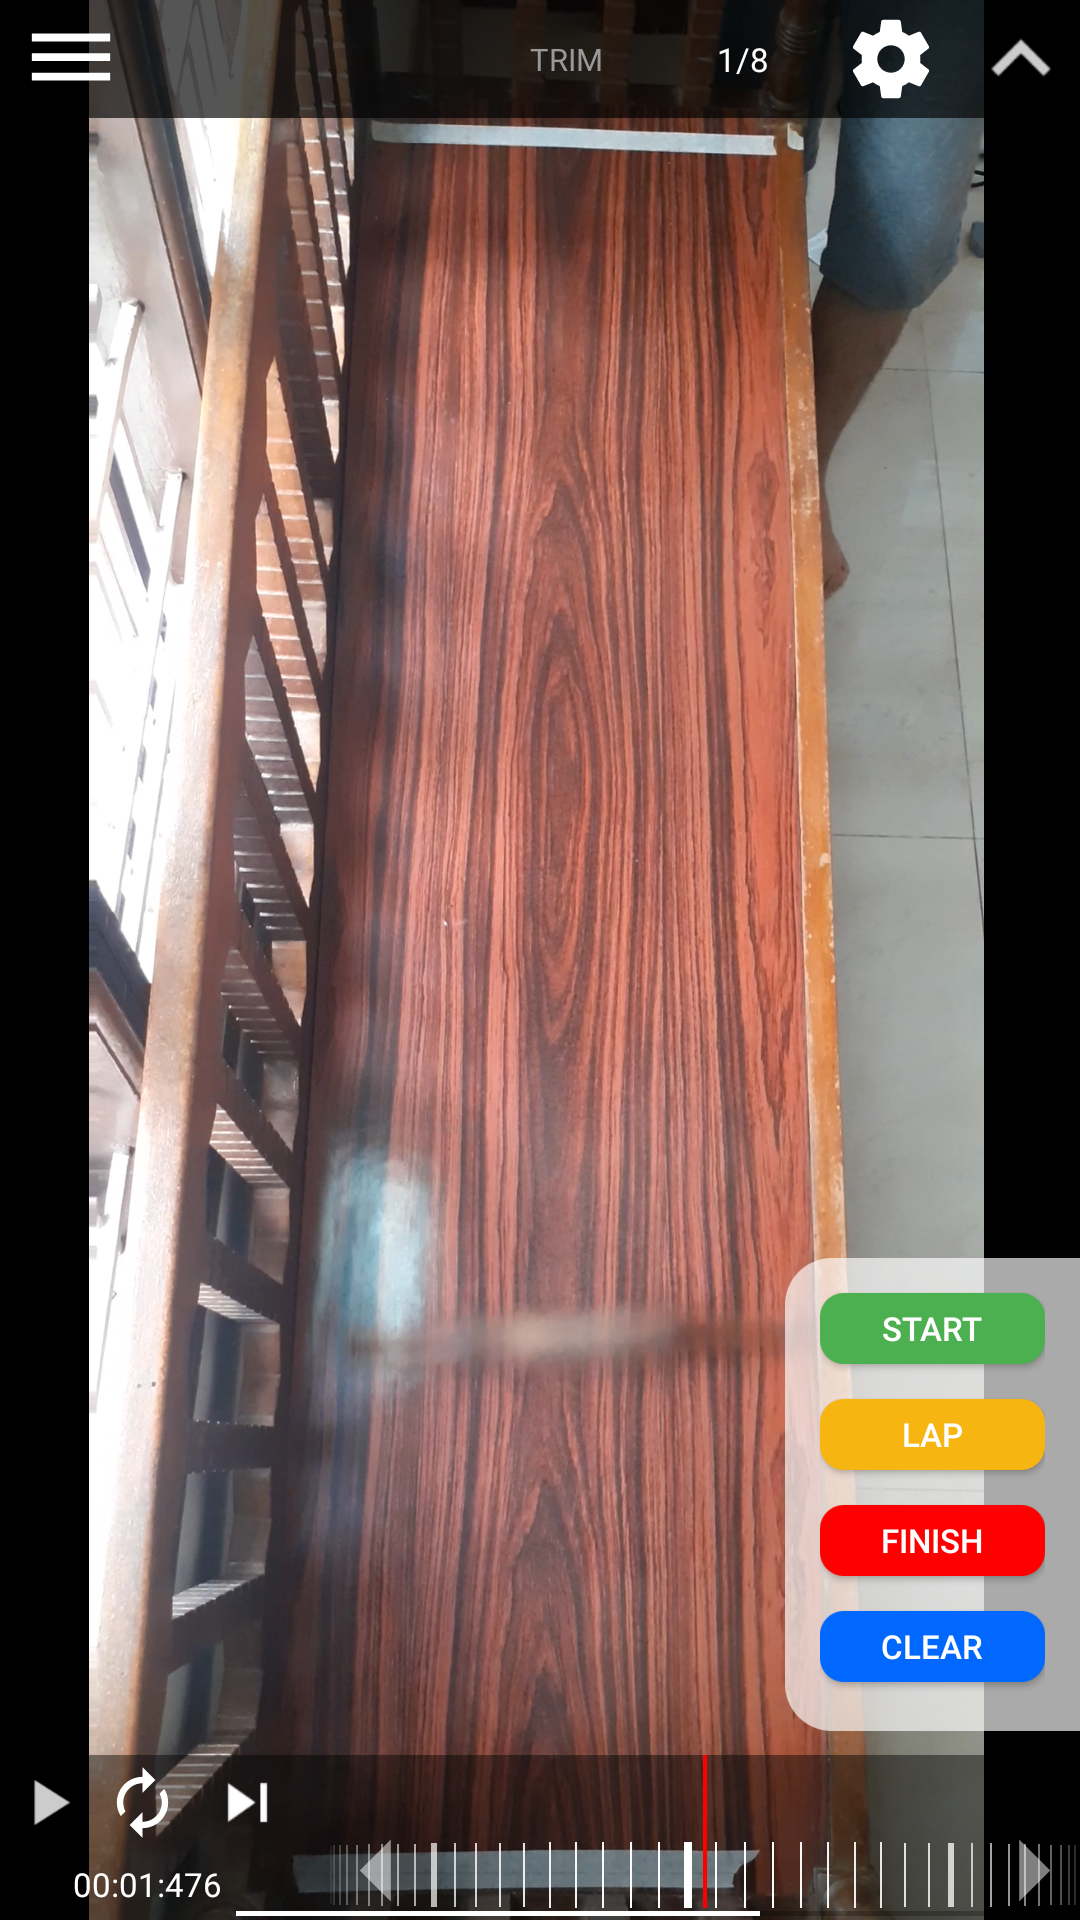
\includegraphics[width=0.4\paperwidth]{Videos/Screenshot}

\caption{Screenshot of the app\label{fig:Screeenshot}}
\end{figure}

\begin{table}[H]
\begin{tabular}{l|l|l|l|l|l}
\hline 
Angle(degree) & time (trial1) (in s) & time (trial2) (in s) & time (trial3) (in s) & Mean time (in s) & lift of bench (cm)\tabularnewline
\hline 
2 & 3.5 & 3.433 & 3.433 & 3.455 & 6\tabularnewline
4 & 2.567 & 2.567 & 2.567 & 2.567 & 12\tabularnewline
6 & 2.067 & 2.033 & 2.033 & 2.044 & 18\tabularnewline
8 & 1.733 & 1.8 & 1.767 & 1.767 & 24\tabularnewline
10 & 1.633 & 1.633 & 1.633 & 1.633 & 30\tabularnewline
12 & 1.467 & 1.433 & 1.433 & 1.444 & 35.8\tabularnewline
14 & 1.3 & 1.333 & 1.333 & 1.322 & 41.6\tabularnewline
16 & 1.267 & 1.2 & 1.267 & 1.245 & 47.4\tabularnewline
\end{tabular}

\caption{Measurement of time taken to roll down}
\end{table}

After these sets of measurement, a kitchen anti slip mat was added
on top of the bench surface. The time taken to roll down is measured
again for 6 degree and 8 degree. The time measured thus is 2.033 s
and 1.733 s respectively. This is similar to the one without surface
modification thus rolling time is independent of surface (which is
also clear from the formula for t Eq: \ref{eq:time}).

\subsection{Measurement of weight of belan}

The weight of the belan was calculated using a kitchen weighing scale.The
least count of the used measuring scale was 1g. It was found that
the weight of the belan used in this experiment is 172 $\pm$1 g.

\begin{figure}[H]
\includegraphics[width=0.4\paperwidth]{Videos/BelanWeight}

\caption{Measurement of weight of belan\label{fig:CircumMeasure-1-1}}
\end{figure}


\subsection{Plots}

Attached outside the report in the form of 2 images.

\subsection{Calculation of moment of inertia of the belan}

From eq \ref{eq:time}
\[
t=\sqrt{\frac{2S(1+I/mR^{2})}{g\sin\theta}}
\]

so 
\[
I=mR^{2}(\frac{t^{2}g\sin\theta}{2S}-1)
\]

let us take R as the weighted mean of $R_{1}$ and$R_{2}$. The weights
can be chosen (assumed) as the fraction of total length that $R_{i}$
appears in the cylinder. The fraction of length with $R_{1}$ is 17/35.8
and that for $R_{2}$ is 18.8/35.8.

Thus R using these weights become $\frac{aR_{1}+bR_{2}}{a+b}=1.28\pm(0.01+0.02)=1.28\pm0.03$cm.

Using theses values and the vales from 2 degree angle data, and g=9.81m$/s^{2}$
we calculate I as 0.0000074312 Kg$m^{2}$ = 74.312 g$cm^{2}$

\[
\frac{\Delta I}{I}=\frac{\Delta m}{m}+2\frac{\Delta R}{R}+2\frac{\Delta t}{t}+cos\theta\Delta\theta+\frac{\Delta S}{S}
\]
 calculating these with the previously mentioned error fractions,

\[
\frac{\Delta I}{I}=0.073410
\]

\[
\Delta I=0.00000054552Kgm^{2}=5.45gcm^{2}
\]

Therefore I = 74.312 $\pm5.45gcm^{2}$.

\subsection{Calculation of coefficient of friction }

In the limiting case where frictional force can no longer support
rolling of the cylinder, thus the cylinder begins to slip. In my case
the $\theta max$was found to be 55 degree. Using eq\ref{eq:mu} 
\[
\mu=\frac{I\tan\theta_{max}}{mR^{2}+I}
\]

we get $\mu=0.298\sim0.3$

\[
\frac{\Delta\mu}{\mu}=\frac{\Delta I}{I}+2\frac{\Delta R}{R}+\frac{\Delta m}{m}+cot\theta\Delta\theta
\]

\[
\frac{\Delta\mu}{\mu}=0.15473
\]

Therefore $\Delta\mu=0.046,$thus $\mu=0.298\pm0.046$

\section{Results \& Conclusion}
\begin{enumerate}
\item The moment of inertia of belan is found to be 74.312 $\pm5.45gcm^{2}$
\item The relation ship between rolling time and the inclination angle is
$t=\sqrt{\frac{2S(1+I/mR^{2})}{g\sin\theta}}$
\item The coefficient of friction of the surface is found to be $\mu=0.298\pm0.046$.
\item The rolling time is independent of surface friction (as long as $f_{s}>mg\sin\theta$).
\end{enumerate}

\end{document}
